\setcounter{section}{0}%更改chapter的计数器值
%\numberwithin{equation}{chapter}%公式计数器从属于节计数器
\numberwithin{equation}{section}%公式计数器从属于节计数器
\numberwithin{figure}{section}%图计数器从属于节计数器
\setcounter{chapter}{2}

%\chapter{\texorpdfstring{Polyakov路径积分}{3 The Polyakov path integral}}
\chapter{Polyakov路径积分}
我们现在用Polyakov路径积分和共形场论对弦论做一系统研究. 在介绍路径积分绘景后,我们讨论规范固定,Weyl反常与顶点算符,之后我们将弦论推广至弯曲时空.
%\section{\texorpdfstring{世界面上的求和}{3.1 Sums over world-sheets}}
\section{世界面上的求和}
Feynman路径积分是表示量子论的一种方法,并且它是描述弦论中相互作用的一个非常自然的方法. 在路径积分量子化中,振幅通过对初态和末态之间所有可能插入的历史求和获得. 每个历史被赋予权重
\begin{equation}
	\exp \left(i S_{\mathrm{cl}} / \hbar\right)
\end{equation}
其中$S_{cl}$是该给定历史的经典作用量. 因此,对连接给定初始曲线与终末曲线的所有世界面求和,将定义弦论中的振幅. 图(\ref{Fig3.1}a) 是针对开弦,图(\ref{Fig3.1}b) 是针对闭弦.\\
\begin{figure}
	\begin{center}
		%width=0.8\textwidth,bb=0 0 680 374
		%1px=0.75pt
		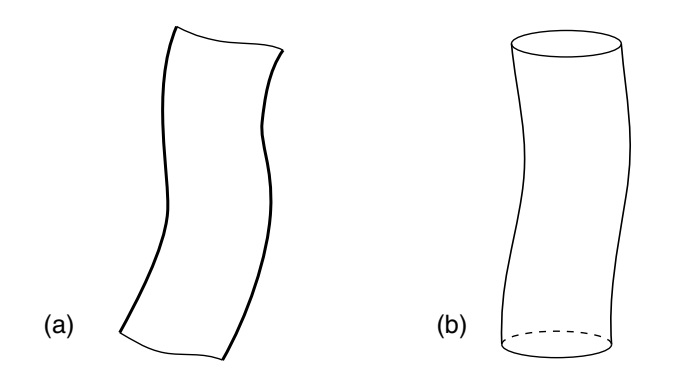
\includegraphics[width=0.8\textwidth,natwidth=500,natheight=240]{Fig3.1.jpg}\\
\caption{(a) An open string world-sheet with the topology of a strip. The heavier curves are the world-lines of string endpoints. (b) A closed string world-sheet with the topology of a cylinder.}\label{Fig3.1}
	\end{center}
\end{figure}
对相对论点粒子的类似求和产生自由传播子.\\
可以想象出弦相互作用的数个方法. 一种是连接相互作用,两弦相交时的能量;另一种是经由某种量子场的长程力. 然而我们在弦论中增加的相互作用不可能与对称性相容;稍后我们将明白为什么是这样的原因. 相反,唯一允许的相互作用是那些已经隐含在世界面求和中的相互作用. 例如考察图(\ref{Fig3.2}) 所示的世界面.\\
\begin{figure}
	\begin{center}
		%width=0.8\textwidth,bb=0 0 741 390
		%1px=0.75pt
		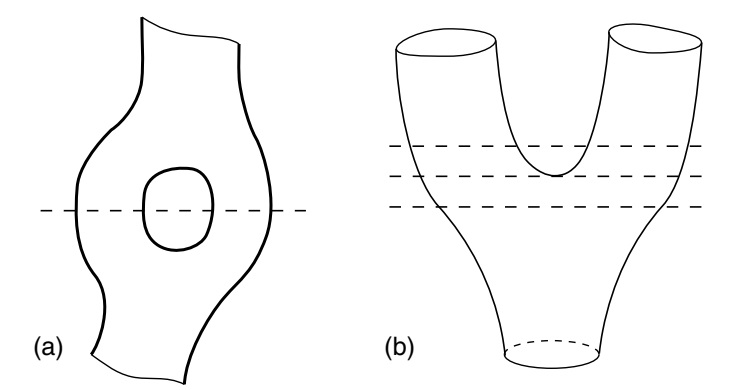
\includegraphics[width=0.75\textwidth,natwidth=500,natheight=218]{Fig3.2.jpg}\\
\caption{(a) Quantum correction to open string propagation. (b) Decay of one closed string into two. The dashed lines are time-slices.}\label{Fig3.2}
	\end{center}
\end{figure}
图(\ref{Fig3.2}a)看起来是对图(\ref{Fig3.1}a)开弦振幅的量子修正. 这个修正包含一个有两个开弦的中间态. 图(\ref{Fig3.2}b)有三个外闭弦并代表一个弦衰变成两个弦. 从中看出这是在弦中引入相互作用的一种正确方式. 我们将看到这些相互作用产生了包含引力的相容理论,有限且幺正.
像图(\ref{Fig3.3})那样在连续的几个时刻里考察图(\ref{Fig3.2}b)的过程是很有趣的.\\
\begin{figure}
	\begin{center}
		%width=0.8\textwidth,bb=0 0 510 279
		%1px=0.75pt
		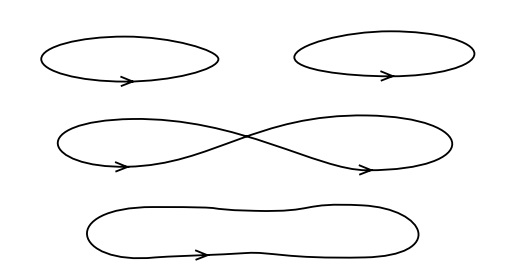
\includegraphics[width=0.65\textwidth,natwidth=350,natheight=138]{Fig3.3.jpg}\\
\caption{Successive time-slices from figure 3.2(b). The arrows indicate the orientation of the string.}\label{Fig3.3}
	\end{center}
\end{figure}
在闭弦理论中,所有粒子作为弦的不同激发态获得. 而所有的相互作用(规范,引力,Yukawa)源于图(\ref{Fig3.3})的单个过程.\\
对于有开弦的理论,存在几种额外能够发生的过程,如图(\ref{Fig3.4}) 所示.\\
\begin{figure}
	\begin{center}
		%width=0.8\textwidth,bb=0 0 783 471
		%1px=0.75pt
		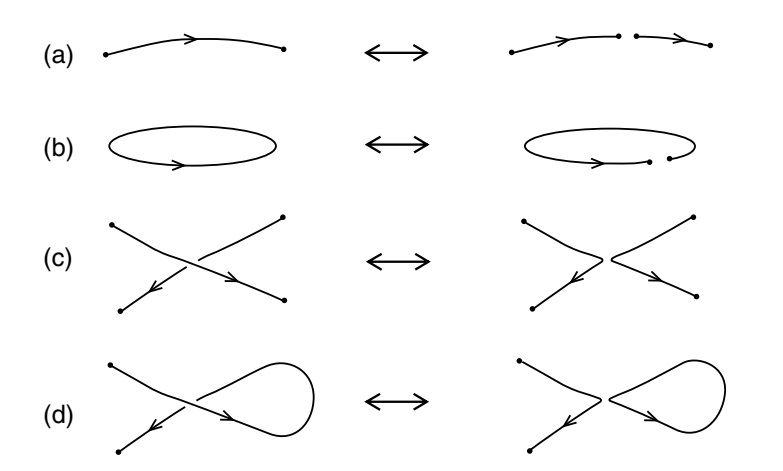
\includegraphics[width=0.7\textwidth,natwidth=520,natheight=250]{Fig3.4.jpg}\\
\caption{Processes involving open strings: (a) open ↔ open + open; (b) closed↔ open; (c) open + open ↔ open + open; (d) open ↔ open + closed.}\label{Fig3.4}
	\end{center}
\end{figure}
在一给定时刻,图(\ref{Fig3.3})与图(\ref{Fig3.4})发生在确定的时空点,但这是一个错觉. 一个不同剪切(slicing),在推动(boosted)Lorentz系中,将显然的相互作用放在不同点上;在时空中不存在可区分的点. 相互作用仅源于世界面的整体拓扑,而世界面的定域性质在自由情况下是相同的. 正如导论中所讨论的,这一点涂抹出来的相互作用截断了引力的短距发散. \\
实际上还有几种不同的弦论,依赖于我们在世界面求和中引入的拓扑. 注意到我们所画的世界面有两类边界,源边界对应初态与末态的弦构型,而端点边界对应开弦端点的世界线. 现在忽视源边界,我们将在本章后面讨论源的细节. 所以在之后的讨论中,“边界”意味着端点边界. 那么有4种方式定义对世界面求和,对应1.4节末尾所列的4种自由弦理论:
\begin{enumerate}
	\item 闭定向:所有无边界的定向世界面;
	\item 闭非定向:所有无边界的世界面;
	\item 闭加开定向:有任意个边界的所有定向世界面;
	\item 闭加开非定向:有任意个边界的所有世界面;
\end{enumerate} 
我们在这里要详述两件事. 其一是非定向世界面内含物之间的连结以及1.4节所描述的$\Omega=+1$投影. 图(\ref{Fig3.5})展示了计入开弦非定向理论的两个世界面.\\
\begin{figure}
	\begin{center}
		%width=0.8\textwidth,bb=0 0 717 409
		%1px=0.75pt
		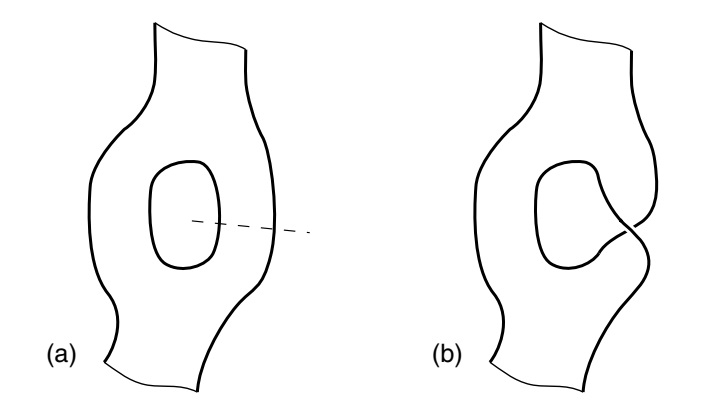
\includegraphics[width=0.65\textwidth,natwidth=500,natheight=230]{Fig3.5.jpg}\\
\caption{Oriented (a) and unoriented (b) contributions to the two-open-string amplitude.}\label{Fig3.5}
	\end{center}
\end{figure}
图(\ref{Fig3.5}b)的世界面等价于沿着虚线剪断图(\ref{Fig3.5}a)的定向世界面. 我们用$0 \leq \sigma \leq \pi$参量化它,并要求在剪断处的场满足
\begin{equation}
X_{\text {upper }}^{\mu}(\sigma)=X_{\text {lower }}^{\mu}(\pi-\sigma)
\end{equation}
这反过来等价于用算符$\Omega$作用在开弦态上. 将这两个平面赋予合适的权重加起来,那么相当于插入算符$\frac{1}{2}(1+\Omega)$,其投射到
$\Omega=+1$的态上. 在对所有定向曲面与非定向曲面的求和中,在所有中间态上插入投影算符,将频谱约化至$\Omega=+1$部分.\\
其二,之上的列表中没有计入只有开弦的理论. 我们来细致地解释下为什么是这种情况.\\
\begin{figure}
	\begin{center}
		%width=0.8\textwidth,bb=0 0 740 280
		%1px=0.75pt
		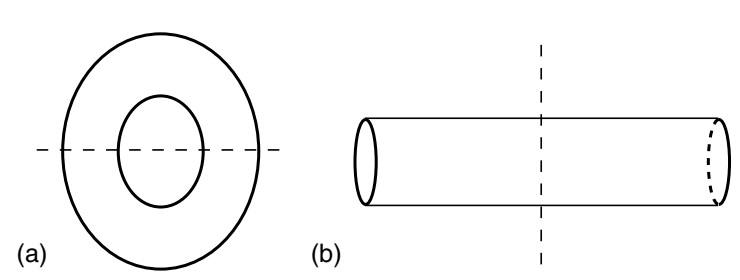
\includegraphics[width=0.8\textwidth,natwidth=520,natheight=190]{Fig3.6.jpg}\\
\caption{(a) An annulus: the intermediate state is two open strings. (b) The same topology drawn as a cylinder: the intermediate state is one closed string.}\label{Fig3.6}
	\end{center}
\end{figure}
考察一个拓扑为圆环的世界面,如图(\ref{Fig3.6}a). 方便起见,我们只画出了真空振幅,但通过连上合适的源,相同的讨论也适用于散射振幅. 从虚线中可以看出这是一个中间态有两个开弦的过程. 因而这类拓扑的世界面必须出现在有开弦的任何理论中. 在图(\ref{Fig3.6}b),我们将同一拓扑画成圆柱,并在单个闭弦的中间态上切开它. 因此,即使我们只从闭弦出发,对世界面的求和将必然地引入这样的过程——开弦的散射产生闭弦. 随着振幅的发散,我们将细致地看到它是如何运作的.\\
开弦理论中闭弦的需求可以从另一方面看到. 考察图(\ref{Fig3.4}ab)中的相互作用,但时间反演:两个开弦合并成一个,一个开弦变成闭弦. 在相互作用点附加它们是相同的,两个端点合并为了有第一个相互作用而没有第二个. 将要求在弦的动力学上附加某些非定域约束;这将确认是不相容的. 可以对图(\ref{Fig3.4}cd)作同一讨论,其中相互作用定域的是一对弦的重新连接,因而,如果任何开弦相互作用被允许了,那么在开弦产生闭弦的同一过程也是允许的.

\section{Polyakov路径积分}%{3.2 The Polyakov path integral}

我们现在开始发展对世界面的求和. 其为对Polyakov形式体系的场积分. 我们这里与第1章有个区别:Minkowski度规$\gamma_{ab}$被替换为奇异性为(+,+)的Euclid度规$g_{a b}\left(\sigma^{1}, \sigma^{2}\right)$,积分取遍所有的Euclid度规以及世界面在Minkowski时空中的嵌入$X^{\mu}\left(\sigma^{1}, \sigma^{2}\right)$:
\begin{equation}\label{3.2.1}
\int[d X d g] \exp (-S)
\end{equation}
Euclid作用量是
\begin{equation}
S=S_{X}+\lambda \chi
\end{equation}
其中
\begin{subequations}\label{3.2.3}
\begin{equation}
S_{X}=\frac{1}{4 \pi \alpha^{\prime}} \int_{M} d^{2} \sigma g^{1 / 2} g^{a b} \partial_{a} X^{\mu} \partial_{b} X_{\mu}
\end{equation}
\begin{equation}
\chi=\frac{1}{4 \pi} \int_{M} d^{2} \sigma g^{1 / 2} R+\frac{1}{2 \pi} \int_{\partial M} d s k
\end{equation}
\end{subequations}
这里ds是沿着边界的固有时,k是边界的测地线曲率,$k=\pm t^{a} n_{b} \nabla_{a} t^{b}$.
$t^a$ 是切于边界的单位向量,而$n^a$ 是向外垂直于$t^a$ 的单位矢量,+号对应类时边界,-对应类空边界. 在这里边界总是类空的. Euclid路径积分的优点是对度规的积分可以更好地定义. 我们所描述的拓扑非平庸世界面可以有非奇异的Euclid度规,而Minkowski度规不行. 我们将取Euclid理论(\ref{3.2.1})作为出发点. 我们将证明如何给它一个精准的定义并且它所定义的相容时空理论. 然而,我们将给出一个简要的形式讨论,它等价于我们出发点Minkowski理论. \\
我们从点粒子的例子出发,其中路径积分
\begin{equation}
\int[d \eta d X] \exp \left[\frac{i}{2} \int d \tau\left(\eta^{-1} \dot{X}^{\mu} \dot{X}_{\mu}-\eta m^{2}\right)\right]
\end{equation}
是振荡的. 对$\eta, X^\mu$ 的路径积分是普通积分的乘积,因而我们可以像普通积分那样对围道变形. 如果我们取
\begin{equation}
\eta(\tau) \rightarrow e^{-i \theta} \eta(\tau), \quad X^{0}(\tau) \rightarrow e^{-i \theta} X^{0}(\tau)
\end{equation}
对于无限小的$\theta$,指数中的所有项要求有一负的实部,使其作为收敛因子. 现在我们可以在场空间中旋转围道$\eta=-i e, X^{0}=-i X^{D}$ ,积分变成
\begin{equation}
\int[d e d X] \exp \left[-\frac{1}{2} \int d \tau\left(e^{-1} \sum_{\mu=1}^{D} \dot{X}^{\mu} \dot{X}^{\mu}+e m^{2}\right)\right]
\end{equation}
这是路径积分(\ref{3.2.1})的Euclid点粒子类比. 我们仅仅做了一个围道旋转. 所以Euclid路径积分给出与Minkowski相同的振幅. \\
如果我们将度规写成四元基的形式$\gamma_{a b}=-e_{a}^{0} e_{b}^{0}+e_{a}^{1} e_{b}^{1}$,并在$e_a^0$上做同一旋转,相同的处理适用于Polyakov作用量. 这提供了Minkowski路径积分与Euclid路径积分等效的一个形式证明. 通过显式的计算,在光锥规范荷共形规范下分别证明了它们有相同的振幅.\\
在(\ref{3.2.3}a)中我们留下了$X^0$的旋转,这是为了强调时空的Minkowski特性. 写成了$X^0$的形式,运动方程与OPE是协变的,度规为$\eta^{\mu\nu}$. \\
我们注意到在二维中,$\chi$定域地是全导数,因而反依赖于世界面的拓扑——它是世界面的Euler数. 因而,$e^{-\lambda \chi}$因子在路径积分中只影响世界面求和中不同拓扑的相对权重. 如果我们向世界面中增加额外的带,就像我们从图(\ref{Fig3.1}a)到图(\ref{Fig3.2}a)中做的那样,Euler数减1,路径积分被赋予额外的权重$e^\lambda$. \\
由于增加一个带对应于发射并再吸收一个虚开弦,从任意过程中发射一个开弦的振幅正比于$e^{\lambda/2}$. 在任意世界面上增加一个把手将Euler数减2,因而增加因子$e^{2\lambda}$.  由于这对应发射和再吸收一个闭弦,发射一个闭弦的振幅正比于$e^\lambda$. 作用量中的Euler项因而控制着弦论中的耦合常数. 其中
\begin{equation}\label{3.2.7}
g_{\mathrm{o}}^{2} \sim g_{\mathrm{c}} \sim e^{\lambda}
\end{equation}
附带的,$\lambda$可以视为理论中的自由参量. 这与绪论中弦论没有这种参量的陈述矛盾. 这是一个关键点,我们将在3.7节解决它.\\
另一方面,耦合的计数以一种简单的方式扩张到世界面与弦源. 闭弦的源是闭边界的,开弦的源是有边界的线段. 方便起见,我们将要求开弦源边界与端点边界在是界面度规下直角. 我们必须小心,因为边界曲率在角处发散. Euler数是
\begin{equation}
\chi=\tilde{\chi}+\frac{1}{4} n_{\mathrm{c}}
\end{equation}
其中 仅包括光滑边界部分上的积分. $n_C$是角的树木. 路径积分正确的权重是
\begin{equation}\label{3.2.9}
\exp (-\lambda \tilde{\chi})=\exp \left(-\lambda \chi+\lambda n_{\mathrm{c}} / 4\right)
\end{equation}
这源于幺正性:如果我们剪开世界面,$\lambda$相关性必须不变. 对于权重(\ref{3.2.9}) 正是这种情况.
这是因为在$\tilde{\chi}$中的面积分在边缘处抵消了. 增加一个闭弦源相当于在世界面上剪了个洞,并将$\chi$减1. 增加开弦源使$\chi$不变但$n_c$加2. 因而,我们得到了发射闭弦或开弦的振幅,这与(\ref{3.2.7}相同). 

\section{规范固定}%{3.3 Gauge fixing}

路径积分(\ref{3.2.1})不是完全正确的,它包含一个庞大的重复计数. 这是因为构型$(X, g)$与 $\left(X^{\prime}, g^{\prime}\right)$若通过diff $\times$ Weyl对称性相关,则代表同一物理构型. 事实上我们需要除以定域对称群的体积
\begin{equation}\label{3.3.1}
\int \frac{[d X d g]}{V_{\text {diff } \times \text { Weyl }}} \exp (-S) \equiv Z
\end{equation}

我们将通过规范固定实现这一点.  对穿过每一个规范等价类一次薄片积分, 并通过 Faddeev - Popov 方法获得薄片上的正确测度. \\
在第1章,我们附加了光锥规范.  这由于某些原因是有用的,但隐藏了理论的某些对称性,所以我们现在做另一选择. 注意到度规是对称的,有三个独立分量,并存在三个规范函数,两个坐标与度规的定域缩放. 因此恰好存在足够多的规范自由度以消除度规上的积分. 将其固定在某个特定的泛函形式,我们称其为基准度规
\begin{equation}
g_{a b}(\sigma) \rightarrow \hat{g}_{a b}(\sigma)
\end{equation}
一个简单的选择是平坦度规或单位规范度规
\begin{equation}\label{3.3.3}
\hat{g}_{a b}(\sigma)=\delta_{a b}
\end{equation}
有时希望单独考虑diff群的效应. 我们可以将任意度规变成单位形式的一个Weyl变换,这是共形规范
\begin{equation}
\hat{g}_{a b}(\sigma)=\exp [2 \omega(\sigma)] \delta_{a b}
\end{equation}
这样,任何度规至少可以定域地变成平坦形式. 首先,做一Weyl变换以使Ricci标量为零. Ricci标量的Weyl变换
\begin{equation}\label{3.3.5}
g^{\prime 1 / 2} R^{\prime}=g^{1 / 2}\left(R-2 \nabla^{2} \omega\right)
\end{equation}
令$R^{\prime}=0$ 要求解 $2 \nabla^{2} \omega=R$. 这总是可能的. 类似于静电学中的讨论. 在二维中,Ricci标量为零暗示着Riemann张量为零,因为Riemann张量的对称性暗示
\begin{equation}
R_{a b c d}=\frac{1}{2}\left(g_{a c} g_{b d}-g_{a d} g_{b c}\right) R
\end{equation}
所以度规是平坦的,且坐标等价于单位度规(\ref{3.2.3}).\\
在这里像第2章中那样引入复坐标$z=\sigma^{1}+i \sigma^{2}$,平坦度规$d s^{2}=d z d \bar{z}$. 考察一个坐标变换,使得$z^\prime$是z的全纯函数
\begin{equation}\label{3.3.7}
z^{\prime} \equiv \sigma^{\prime 1}+i \sigma^{\prime 2}=f(z)
\end{equation}
结合一个Weyl变换,新度规是
\begin{equation}
d s^{\prime 2}=\exp (2 \omega)\left|\partial_{z} f\right|^{-2} d z^{\prime} d \bar{z}^{\prime}
\end{equation}
那么对于
\begin{equation}\label{3.3.9}
\omega=\ln \left|\partial_{z} f\right|
\end{equation}
这个度规是不变的. 因而,我们还存在一个额外的自由度. diff$\times$Weyl变换.\\
当我们考察整个世界面时,这种额外自由度大多会被消除. 这里存在两个问题. 其一,在Noether定理及Ward等式的讨论中,我们在(2.3.10)下面仔细强调了这些结果依赖于定域定义在世界面上的对称性. 变换(\ref{3.3.7})(\ref{3.3.9})因而会给出守恒流与Ward等式. 这是第2章研究的共形不变性. 我们看到这源于保持单位度规不变的 diff$\times$Weyl子群.\\
第二个问题是当我们确实考察全世界面时,我们对度规和规范自由度的计数发生了什么. 我们将在第5章考虑它们.\\

\centerline{\Large Faddeev-Popov行列式}
在固定度规之后,泛函积分取遍由$X^\mu$参量化的层. 为了获得正确的测度,我们使用Faddeev-Popov步骤. 这个方法与杨-Mills理论中获得的规范固定测度的方法是相同的. 图(\ref{Fig3.7})阐明了这个方法.
\begin{figure}
	\begin{center}
		%width=0.8\textwidth,bb=0 0 654 372
		%1px=0.75pt
		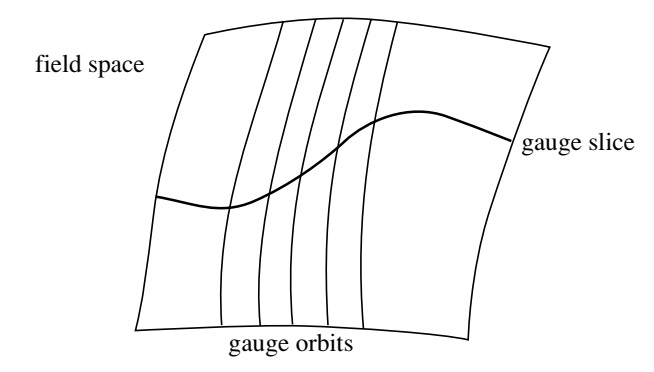
\includegraphics[width=0.8\textwidth,natwidth=490,natheight=279]{Fig3.7.jpg}\\
\caption{Schematic picture of the Faddeev–Popov procedure. The gauge orbits	are families of gauge-equivalent configurations. Integrating over the whole field space and dividing by the orbit volume is equivalent to integrating over a slice that intersects each orbit once, with appropriate Jacobian.}\label{Fig3.7}
	\end{center}
\end{figure}
令$\zeta$ 为坐标变换与Weyl变换的组合
\begin{equation}
\zeta: g \rightarrow g^{\zeta}, \quad g_{a b}^{\zeta}\left(\sigma^{\prime}\right)=\exp [2 \omega(\sigma)] \frac{\partial \sigma^{c}}{\partial \sigma^{\prime a}} \frac{\partial \sigma^{d}}{\partial \sigma^{b}} g_{c d}(\sigma)
\end{equation}
根据标准路线,定义Faddeev-Popov测度$\Delta_{\mathrm{FP}}$
\begin{equation}\label{3.3.11}
1=\Delta_{\mathrm{FP}}(g) \int[d \zeta] \delta(g-\hat{\mathrm{g}} \zeta)
\end{equation}
其中$\hat{\boldsymbol{g}}_{a b}$ 是基准度规. 在(\ref{3.3.11}),$[d \zeta]$是diff $\times$ Weyl群上的规范不变测度. $\delta$函数实际上是 $\delta$泛函. 要求在每一点$g_{a b}(\sigma)=\hat{g}_{a b}^{\zeta}(\sigma)$. 将(\ref{3.3.11})代入泛函积分(\ref{3.3.1})
\begin{equation}
Z[\hat{g}]=\int \frac{[d \zeta d X d g]}{V_{\text {diff } \times \text { Weyl }}} \Delta_{\mathrm{FP}}(g) \delta\left(g-\hat{g}^{\zeta}\right) \exp (-S[X, g])
\end{equation}
进行对$g_{ab}$的积分,并重新命名虚拟变量$X \rightarrow X^{\zeta}$,得
\begin{equation}
Z[\hat{g}]=\int \frac{\left[d \zeta d X^{\zeta}\right]}{V_{\text {diff } \times \text { Weyl }}} \Delta_{\mathrm{FP}}\left(\hat{\mathrm{g}}^{\zeta}\right) \exp \left(-S\left[X^{\zeta}, \hat{\mathrm{g}}^{\zeta}\right]\right)
\end{equation}
现在利用$\Delta_{\mathrm{FP}}$的规范不变性,泛函积分测度[dX]的不变性,以及作用量的规范不变性,得:
\begin{equation}
Z[\hat{\mathrm{g}}]=\int \frac{[d \zeta d X]}{V_{\text {diff } \times \text { Weyl }}} \Delta_{\mathrm{FP}}(\hat{\mathrm{g}}) \exp (-S[X, \hat{\mathrm{g}}])
\end{equation}
\begin{remark}
$\Delta_{\mathrm{FP}}$的规范不变性:
$$
\begin{aligned}
\Delta_{\mathrm{FP}}\left(g^{\zeta}\right)^{-1} &=\int\left[d \zeta^{\prime}\right] \delta\left(g^{\zeta}-\hat{\mathrm{g}} \zeta^{\zeta}\right)=\int\left[d \zeta^{\prime}\right] \delta\left(g-\hat{\mathrm{g}}^{\zeta^{-1} \cdot \zeta^{\prime}}\right) \\
&=\int\left[d \zeta^{\prime \prime}\right] \delta\left(g-\hat{\mathrm{g}}^{\zeta^{\prime \prime}}\right)=\Delta_{\mathrm{FP}}(g)^{-1}
\end{aligned}
$$
其中$\zeta^{\prime \prime}=\zeta^{-1} \cdot \zeta^{\prime} $.
\end{remark}
最后,被积函数中没有什么量依赖于$\zeta$. 所以$\zeta$的积分仅产生了规范群的体积并与分母抵消,留下
\begin{equation}
Z[\hat{g}]=\int[d X] \Delta_{\mathrm{FP}}(\hat{g}) \exp (-S[X, \hat{g}])
\end{equation}
因而$\Delta_{\mathrm{FP}}(\hat{g})$ 是层上的正确测度.\\
为了计算Faddeev-Popov测度的表达式(\ref{3.3.11}),我们假定规范选择完美地固定了规范对称性,使得对于精确的一个$\zeta$值,$\delta(g-\hat{g} ^\zeta)$非零. 而对于$\delta(g-\hat{g}^ \zeta)$这是一个等式. 正如之上所标记的,存在一个整体的小的错误匹配,我们将在时间参与进来时处理它——它不影响世界面的定域性质. 对于接近于1的 $\zeta$,我们可以展开
\begin{equation}
\begin{aligned}
\delta g_{a b} &=2 \delta \omega g_{a b}-\nabla_{a} \delta \sigma_{b}-\nabla_{b} \delta \sigma_{a} \\
&=\left(2 \delta \omega-\nabla_{c} \delta \sigma^{c}\right) g_{a b}-2\left(P_{1} \delta \sigma\right)_{a b}
\end{aligned}
\end{equation}
其中$P_1$是微分算符使矢量成为无迹对称2-张量
\begin{equation}
\left(P_{1} \delta \sigma\right)_{a b}=\frac{1}{2}\left(\nabla_{a} \delta \sigma_{b}+\nabla_{b} \delta \sigma_{a}-g_{a b} \nabla_{c} \delta \sigma^{c}\right)
\end{equation}
在1附近,逆行列式(\ref{3.3.11})变成
\begin{equation}
\begin{aligned}
&\Delta_{\mathrm{FP}}(\hat{\mathrm{g}})^{-1} \\
=&\int[d \delta \omega d \delta \sigma] \delta\left[-(2 \delta \omega-\hat{\nabla} \cdot \delta \sigma) \hat{g}+2 \hat{P}_{1} \delta \sigma\right] \\
=&\int[d \delta \omega d \beta d \delta \sigma] \exp \left\{2 \pi i \int d^{2} \sigma \hat{\mathrm{g}}^{1 / 2} \beta^{a b}\left[-(2 \delta \omega-\hat{\nabla} \cdot \delta \sigma) \hat{g}+2 \hat{P}_{1} \delta \sigma\right]_{a b}\right\} \\
=&\int\left[d \beta^{\prime} d \delta \sigma\right] \exp \left\{4 \pi i \int d^{2} \sigma \hat{\mathrm{g}}^{1 / 2} \beta^{\prime a b}\left(\hat{P}_{1} \delta \sigma\right)_{a b}\right\}
\end{aligned}
\end{equation}
微分算符上的帽子代表它包含基准度规$\hat{g}$. 在第二个等式中,我们使用了泛函$\delta$函数的积分表示. 引入了对称张量场$\beta^{a b} $
,在第三个等式中我们积掉了$\delta \omega$, 其产生了一个delta泛函迫使 $\beta^{a b}$无迹; 那么泛函积分$\left[d \beta^{\prime}\right]$是对无迹对称张量积分. 我们现在有了 $\Delta_{\mathrm{FP}}(\hat{\mathrm{g}})^{-1}$ 作为对矢量场 $\delta \sigma^{a}$ 与无迹对称张量 $\beta^{\prime a b}$的泛函积分表示.\\
通过将Boson场替换为相应的Grassmann鬼场
\begin{subequations}
\begin{equation}
\delta \sigma^{a} \rightarrow c^{a}
\end{equation}
\begin{equation}
\beta_{a b}^{\prime} \rightarrow b_{a b}
\end{equation}
\end{subequations}
我们可以转化路径积分,其中$b^{a b}$像$\beta^{\prime a b}$一样是无迹的. 因而
\begin{equation}
\Delta_{\mathrm{FP}}(\hat{\mathrm{g}})=\int[d b d c] \exp \left(-S_{\mathrm{g}}\right)
\end{equation}
其中,在场的一个方便的归一化下,鬼场作用量是
\begin{equation}\label{3.3.21}
S_{\mathrm{g}}=\frac{1}{2 \pi} \int d^{2} \sigma \hat{g}^{1 / 2} b_{a b} \hat{\nabla}^{a} c^{b}=\frac{1}{2 \pi} \int d^{2} \sigma \hat{g}^{1 / 2} b_{a b}\left(\hat{P}_{1} c\right)^{a b}
\end{equation}
定域地在世界面上,Polyakov路径积分是
\begin{equation}\label{3.3.22}
Z[\hat{g}]=\int[d X d b d c] \exp \left(-S_{X}-S_{\mathrm{g}}\right)
\end{equation}
这个作用量是场的二次型,所以我们可以行列式的形式计算路径积分. 这个计算将在第5章更细致的进行;这里的结果是
\begin{equation}
Z[\hat{g}]=\left(\operatorname{det} \hat{\nabla}^{2}\right)^{-D / 2} \operatorname{det} \hat{P}_{1}
\end{equation}
第一个行列式来自于X积分,而第二个来自于鬼积分.\\
在共形规范下,$\hat{g}_{a b}(\sigma)=\exp [2 \omega(\sigma)] \delta_{a b}$,鬼场作用量(\ref{3.3.21})是
\begin{equation}
\begin{aligned}
S_{\mathrm{g}} &=\frac{1}{2 \pi} \int d^{2} z\left(b_{z z} \nabla_{\bar{z}} c^{z}+b_{\bar{z} \bar{z}} \nabla_{z} c^{\bar{z}}\right) \\
&=\frac{1}{2 \pi} \int d^{2} z\left(b_{z z} \partial_{\bar{z}} c^{z}+b_{\bar{z} \bar{z}} \partial_{z} c^{\bar{z}}\right)
\end{aligned}
\end{equation}
注意,$\omega(\sigma)$并没有出现在最终形式中.  这是因为仅有z指标张量的协变$\bar{z}$导数将简化成简单导数,反之亦然. 读者可以通过解出联络张量来验证这一点. 我们安置了指标,在b的下方和c的上方可以利用这一点. 由于作用量是Weyl不变的,所以
 $b_{a b}$ 和 $c^{a}$ 在左Weyl变换下是中性的 (与 $b^{a b}$和 $c_{a}$相反, 其包含额外的度规因子). 由于共形变换是坐标变换 (3.3.7) 和Weyl变换 (3.3.9)的组合, 我们可以立即从张量指标中读出 $b_{a b}$ 与 $c^{a}$ 的共形变换: 这是 $\left(h_{b}, h_{c}\right)=(2,-1)$的bc CFT 与 $\left(\tilde{h}_{b}, \tilde{h}_{c}\right)=(2,-1)$的$\tilde{b} \tilde{c}$ CFT .\\
我们所给出的规范固定路径积分的推导有时被称为“启发”推导. Polyakov泛函积分(\ref{3.3.1})由于庞大的规范重复计数是病态定义的. 另一方面,规范固定泛函(\ref{3.3.22})的定义是相当好的,并可以清楚地计算出来. 由于实用的原因,我们或许应该视规范固定形式为我们的出发点,而规范不变的那个给了直观解释. 在规范固定形式中,规范对称性的重要内容以BRST不变的形式仍然出现,我们将在下一章开始处理. \\
在开弦中,我们也要考察包含边界线段的部分. 将泛函积分视为固定区域上场的积分是方便的. 所以diff不变性被限制为使边界变换到自身的坐标改变. 因而变分$\delta \sigma^{a}$ 有一零法向分量
\begin{equation}
n_{a} \delta \sigma^{a}=0
\end{equation}
这个边界条件被相应的鬼场
\begin{equation}
n_{a} c^{a}=0
\end{equation}
所继承,所以$c^{a}$正比于切向矢量$t^{a}$. 那么运动方程提供了$b_{a b}$ 上一个边界条件. 它们有表面项
\begin{equation}
\int_{\partial M} d s n^{a} b_{a b} \delta c^{b}=0
\end{equation}
加上$c^a$ 上边界条件. 这暗示了
\begin{equation}
n_{a} t_{b} b^{a b}=0
\end{equation}
这些是我们在2.7节所用的边界条件.

\section{Weyl反常}%{3.4 The Weyl anomaly}


弦论的关键特征之一仅在满足特定条件的时空背景下才是自洽的. 对于平坦时空中的Boson弦论,条件是D=26. 这是作为散射振幅的一个病态首先发现的. 在光锥分析中,它作为Lorentz对称性的一种缺失而产生. 这一约束的潜在原因是定域世界面对称性中的一个反常. 在我们的现代体系中,反常是在Weyl对称性中:${T^a}_a$在经典上为零,但在量子理论中不是. \\
整体Weyl变换,$\omega(\sigma)=$ 常数,等价于长度的总体缩放. 几个四维中的场论在这种缩放下是不变的. 它们包括$\phi^4$无质量标量场论以及非Abel规范场论. 标度不变性是显然的. 这是因为Lagrangian中不包含无量纲参量——每个情况下的耦合常数是无量纲的. 然而,我们知道由于量子理论中的发散,在每个理论中存在一个非零的重整化群$\beta$函数,暗示了有效耦合常数实际上是长度尺度的函数. 相应的,能动量张量的迹在经典理论中为零,但把量子效应考虑进去之后,迹不为零,并正比于$\beta$函数. \\
在上一节,我们忽略了反常的可能性. 我们需要验证它:是否规范固定路径积分Z[g] 真的独立于基准度规的选择
\begin{equation}
Z\left[g^{\zeta}\right]=Z[g] ?
\end{equation}
在4.2节,我们将把这个推广至更普遍的规范变化. 方便起见,此后省略$\hat{g}$上的帽子. 我们也对有额外插入的路径积分感兴趣
\begin{equation}
\langle\ldots\rangle_{g} \equiv \int[d X d b d c] \exp (-S[X, b, c, g]) \ldots
\end{equation}
那么,我们要求
\begin{equation}
\langle\ldots\rangle_{g ^\zeta}=\langle\ldots\rangle_{g}
\end{equation}
当前我们并不对插入的细节感兴趣——那将是下2节的主题. 我们将注意力限制在“...”中的场位置附近$\zeta$为零的规范变换,即,我们疑问Weyl不变性作为算符方程是否成立.\\
很容易保证量子理论中的diff不变性与Poincare不变性. 例如,可以利用Pauli-Villars正规化子定义规范固定路径积分. 将这个路径积分除以一个有质量的正规化场. 有质量正规化子场可以diff不变与Poincare不变方式与度规耦合. 然而,对于一个正规化子场$Y^\mu$,diff不变且Poincare不变的项$\mu^{2} \int d^{2} \sigma g^{1 / 2} Y^{\mu} Y_{\mu}$不是Weyl不变的?任何Weyl变换可作为无限小变换重复的结果而获得. 所以研究后者就足够了.\\
能动量张量$T^{\mu\nu}$是路径积分相对于度规的无穷小变分
\begin{equation}\label{3.4.4}
\delta\langle\ldots\rangle_{g}=-\frac{1}{4 \pi} \int d^{2} \sigma g(\sigma)^{1 / 2} \delta g_{a b}(\sigma)\left\langle T^{a b}(\sigma) \ldots\right\rangle_{g}
\end{equation}
经典上,$T^{\mu\nu}$完全来自作用量的变分,并且这与Noether定义一致
\begin{equation}
T^{a b}(\sigma) \stackrel{\text { classical }}{=} \frac{4 \pi}{g(\sigma)^{1 / 2}} \frac{\delta}{\delta g_{a b}(\sigma)} S
\end{equation}
它也约化至在平坦世界面极限下的早期定义. 如果取$\delta g_{a b}$有坐标变换的形式,路径积分的diff不变性暗示$T^{ab}$守恒.\\
在下面的分析中,我们将先忽略可能的边界项,对于一个Weyl变换$T^{ab}$的定义(\ref{3.4.4}) 意味着
\begin{equation}\label{3.4.6}
\delta_{\mathrm{W}}\langle\ldots\rangle_{g}=-\frac{1}{2 \pi} \int d^{2} \sigma g(\sigma)^{1 / 2} \delta \omega(\sigma)\left\langle T_{a}^{a}(\sigma) \ldots\right\rangle_{g}
\end{equation}
所以在普遍插入“...”,Weyl不变性可以表述为算符陈述:能动量张量是无迹的
\begin{equation}
{T^a}_{a} \stackrel{?}{=} 0
\end{equation}
经典作用量是Weyl不变的,但在量子理论中,由于我们还没发现一个完全的规范不变正规化子,这个迹可能非零. 这个迹必须是diff不变且Weyl不变的,因为我们保护了这些对称性. 它在平坦时空中为零. 因为我们从上一章知道了这个理论是共形平坦的,这仅留下一种可能性:
\begin{equation}\label{3.4.8}
{T^a}_{a}=a_{1} R
\end{equation}
a为某个常数. R又一次是世界面Ricci标量. 带有超过两个导数的项由于量纲的原因而被禁止. 在世界面长度的单位下,$g_{ab}, X^\mu$都是无量纲的. 所以(\ref{3.4.8})中的常数$a_1$也是无量纲的. 带有多个导数的项将有一个系数,这个系数有着用来定义路径积分的截断长度量纲的正幂次,所以在截断取为零的极限下为零.\\

\centerline{\Large Weyl反常的计算}
构建规范不变理论中可能的障碍已经退化至单个常数$a_1$. 事实上,这个数正比于我们计算过的一个量——平坦世界面上CFT的中心荷c. $a_1, c$均与能动量张量的两点函数有关,尽管是与不同的分量. 为了得到它们间的精确关系, 我们将需要使用diff不变性. 在(复坐标)共形规范下
\begin{equation}
T_{z \bar{z}}=\frac{a_{1}}{2} g_{z \bar{z}} R
\end{equation}
取协变导数
\begin{equation}
\nabla^{\overline{z}} T_{\bar{z} z}=\frac{a_{1}}{2} \nabla^{\bar{z}}\left(g_{z \bar{z}} R\right)=\frac{a_{1}}{2} \partial_{z} R
\end{equation}
其中我们使用了度规是协变导数的事实. 那么$T_{ab}$的守恒
\begin{equation}\label{3.4.11}
\nabla^{z} T_{z z}=-\nabla^{\bar{z}} T_{\bar{z} z}=-\frac{a_{1}}{2} \partial_{z} R
\end{equation}
为了固定$a_1$,我们比较左边和右边的Weyl变换. 右边的Weyl变换(\ref{3.3.5})
\begin{equation}\label{3.4.12}
a_{1} \partial_{z} \nabla^{2} \delta \omega \approx 4 a_{1} \partial_{z}^{2} \partial_{\bar{z}} \delta \omega
\end{equation}
其中我们在一个平坦的世界面附近展开. 为了得到$T_{zz}$上的Weyl变换,我们首先使用共形变换
\begin{equation}
\epsilon^{-1} \delta T_{z z}(z)=-\frac{c}{12} \partial_{z}^{3} v^{z}(z)-2 \partial_{z} v^{z}(z) T_{z z}(z)-v^{z}(z) \partial_{z} T_{z z}(z)
\end{equation}
从3.3节中的讨论,这个共形变换由一个坐标变换
of a coordinate transformation $\delta z=\epsilon v$ 加上一个Weyl变换 $2 \delta \omega=\epsilon \partial v+\epsilon(\partial v)^{*}$构成. 变分中的后两项是张量的坐标变换,所以Weyl变换至平坦空间的领头阶是
\begin{equation}
\delta_{\mathrm{W}} T_{z z}=-\frac{c}{6} \partial_{z}^{2} \delta \omega
\end{equation}
用$\partial^{z}=2 \partial_{\bar{z}}$作用,并与变换(\ref{3.4.12})相比给出:
\begin{equation}\label{3.4.15}
c=-12 a_{1}, \quad {T^a}_{a}=-\frac{c}{12} R
\end{equation}
\begin{proof}
$$
\partial^{z} \delta_{W} T_{z z}=2\left(-\frac{c}{6}\right) \partial_{\bar{z}} \partial_{z}^{2} \delta \omega
$$
$$
(3.4.12)right. hand=4 a_{1} \partial_{z}^{2} \partial_{\bar{z}} \delta \omega
$$
\end{proof}
我们用另一个稍长一点的步骤再推导一次. 其中,我们会得到一个有用的中间结果. 在共形规范下
\begin{subequations}\label{3.4.16}
\begin{equation}
R=-2 \exp (-2 \omega) \partial_{a} \partial_{a} \omega
\end{equation}
\begin{equation}
\nabla^{2}=\exp (-2 \omega) \partial_{a} \partial_{a}
\end{equation}
\end{subequations}
通过收缩两个下指标,亦即$\delta^{a b} \partial_{a} \partial_{b}$,Z[g]的Weyl变分(\ref{3.4.6})是
\begin{equation}
\delta_{\mathrm{W}} Z[\exp (2 \omega) \delta]=\frac{a_{1}}{\pi} Z[\exp (2 \omega) \delta] \int d^{2} \sigma \delta \omega \partial_{a} \partial_{a} \omega
\end{equation}
其中$\exp (2 \omega) \delta$ 代表共形规范,积分立即给出
\begin{equation}\label{3.4.18}
Z[\exp (2 \omega) \delta]=Z[\delta] \exp \left(-\frac{a_{1}}{2 \pi} \int d^{2} \sigma \partial_{a} \omega \partial_{a} \omega\right)
\end{equation}
由于每个度规diff等价于共形度规. (\ref{3.4.18})实际上决定了Z[g]的全部度规依赖性. 我们需要找到diff不变表达式. 其在共形规范下退化至(\ref{3.4.18}). 利用(\ref{3.4.16}) 可以证明期望的表达式是:
\begin{equation}\label{3.4.19}
Z[g]=Z[\delta] \exp \left[\frac{a_{1}}{8 \pi} \int d^{2} \sigma \int d^{2} \sigma^{\prime} g^{1 / 2} R(\sigma) G\left(\sigma, \sigma^{\prime}\right) g^{1 / 2} R\left(\sigma^{\prime}\right)\right]
\end{equation}
其中
\begin{equation}
g(\sigma)^{1 / 2} \nabla^{2} G\left(\sigma, \sigma^{\prime}\right)=\delta^{2}\left(\sigma-\sigma^{\prime}\right)
\end{equation}
定义了标量Green函数. 这是一个有趣的结果:路径积分完全由反常方程决定.\\
现在围绕平坦背景展开$Z[g]$ , $g_{a b}=\delta_{a b}+h_{a b}$, 并保留 $h_{\bar{z} \bar{z}} $的二阶项. Ricci 标量是 $4 \partial_{z}^{2} h_{\bar{z} \bar{z}}$ (到 $h_{\bar{z} \bar{z}}$的一阶), 所以忽略收缩项,其中 $z=z^{\prime}$ 
\begin{equation}\label{3.4.21}
\begin{aligned}
\ln \frac{Z[\delta+h]}{Z[\delta]} & \approx \frac{a_{1}}{8 \pi^{2}} \int d^{2} z \int d^{2} z^{\prime}\left(\partial_{z}^{2} \ln \left|z-z^{\prime}\right|^{2}\right) h_{\bar{z} \bar{z}}(z, \bar{z}) \partial_{z^{\prime}}^{2} h_{\bar{z} \bar{z}}\left(z^{\prime}, \bar{z}^{\prime}\right) \\
&=-\frac{3 a_{1}}{4 \pi^{2}} \int d^{2} z \int d^{2} z^{\prime} \frac{h_{\bar{z} \bar{z}}(z, \bar{z}) h_{\bar{z} \bar{z}}\left(z^{\prime}, \bar{z}^{\prime}\right)}{\left(z-z^{\prime}\right)^{4}}
\end{aligned}
\end{equation}
我们可以用度规中的二阶微扰论计算它. 其通过(\ref{3.4.4})给出:
\begin{equation}
\ln \frac{Z[\delta+h]}{Z[\delta]} \approx \frac{1}{8 \pi^{2}} \int d^{2} z \int d^{2} z^{\prime} h_{\bar{z} \bar{z}}(z, \bar{z}) h_{\bar{z} \bar{z}}\left(z^{\prime}, \bar{z}^{\prime}\right)\left\langle T_{z z}(z) T_{z z}\left(z^{\prime}\right)\right\rangle_{\delta}
\end{equation}
现在使用标准TTOPE(2.4.25). 除了第一个包含非零自旋算符的项,所有的项由于旋转不变性为零. 留下$\left\langle T_{z z}(z) T_{z z}\left(z^{\prime}\right)\right\rangle_{\delta}=\frac{1}{2} c\left(z-z^{\prime}\right)^{-4}$.
与从Weyl反常得到的结果(\ref{3.4.21})相比,又一次给出(\ref{3.4.15}).

\centerline{\Large 讨论}
由$X^\mu$,中心荷D及鬼构成的世界面理论,给出
\begin{equation}
c=c^{X}+c^{\mathrm{g}}=D-26
\end{equation}
其中,鬼的中心荷(2.5.12)是-26. 这个理论仅对D=26是Weyl不变的,与第1章发现的Lorentz不变性的条件相同. 当Weyl反常不为零,不同的规范选择是不等价的. 并且就像带有反常的规范理论,任何一个选择导致了一个病态,诸如协变性或幺正性的缺失. 例如,在光锥规范下,选择不同的时空轴要求了规范的范围,所以潜在的Weyl反常转变成了Lorentz反常.\\
还有另一件事可以尝试:忽视Weyl反常,仅将diff不变性视为规范对称性. 那么度规将有一个实自由度$\omega(\sigma)$要被积掉而不是规范固定. 由于(\ref{3.4.18})中的量子效应对$\omega$所生成的作用就像对$X^\mu$之一的作用;当D>26,这个符号是类空维度的. 然而,物理是有一点小奇怪的,这是因为$\omega$以及随之的能动量张量的diff变换不同于$X^\mu$. 事实上,这个理论是线性伸缩子CFT,所以不存在D+1维Lorentz不变性. 并且这个理论对我们当前目的是无用的,即将物理理解为我们宇宙的一部分. 它是一个有趣的模型,我们将在9.9节简要地回到这点.\\
之上我们发现了当且仅当总中心荷c为零时,一个平坦世界面CFT可以以一种Weyl不变的方式与弯曲度规耦合. 然而,这里存在一个矛盾,由于相同的讨论适用于反全纯中心荷$\tilde{c}$,并且我们已经从bc CFT的例子看出c不需要与$\tilde{c}$相等. 这一点是我们在(\ref{3.4.11})与(\ref{3.4.19})对世界面diff不变性暗中假定过的. 如果$c\neq \tilde{c}$,不存在与$O\left(h_{z z}^{2}\right)$ 和 $O\left(h_{\bar{z} \bar{z}}^{2}\right)$计算均一致的diff不变表达式,那么CFT不能以一种diff不变的方式与弯曲度规耦合;存在diff反常或引力反常. 矛盾表明,一个CFT要想无引力反常,$c= \tilde{c}$是必要的,也可证明它是充分的.

\centerline{\Large 边界的包含}
首先回到方程(\ref{3.4.8}),并考虑更普遍的可能性
\begin{equation}\label{3.4.24}
	T_{a}^{a}=a_{1} R+a_{2}
\end{equation}

这是diff不变性所允许的,但在平坦极限下不为零. 早先我们通过$T_{ab}$的选择(2.3.15b)令$a_2=0$. 等价地,平坦世界面上超过一个守恒$T_{ab}$的存在意味着在我们如何与弯曲度规耦合中存在自由度. 特别地,我们可以附加作用量
\begin{equation}
S_{\mathrm{ct}}=b \int d^{2} \sigma g^{1 / 2}
\end{equation}
这是二维宇宙学常数,它不是Weyl不变的. 它给$T_{ab}$加上了$2 \pi b g_{a b}$,所以迹(\ref{3.4.24})变成
\begin{equation}
T_{a}^{a}=a_{1} R+\left(a_{2}+4 \pi b\right)
\end{equation}
通过令$b=-a_{2} / 4 \pi$,我们可以使第二项为零,这正是我们在(2.3.15b)所做的. $a_2,b$的值依赖于定义,这里不感兴趣.\\
没有可以移除$a_1$的定域抵消项. 例如,$\int d^{2} \sigma g^{1 / 2} R$是Weyl不变的,所以如果$a_1$不为零,在Weyl对称性中存在一个真实的反常. \\
我们现在考察边界的效应. 包含边界项,最普遍的可能变分为
\begin{equation}
\begin{aligned}
\delta_{\mathrm{W}} \ln \langle\ldots\rangle_{\mathrm{g}}=-\frac{1}{2 \pi} & \int_{M} d^{2} \sigma g^{1 / 2}\left(a_{1} R+a_{2}\right) \delta \omega \\
&-\frac{1}{2 \pi} \int_{\partial M} d s\left(a_{3}+a_{4} k+a_{5} n^{a} \partial_{a}\right) \delta \omega
\end{aligned}
\end{equation}

其中又一次地,$k=-t^{a} n_{b} \nabla_{a} t^{b}$是边界的测地曲率. 可能的抵消项是
\begin{equation}
	S_{\mathrm{ct}}=\int_{M} d^{2} \sigma g^{1 / 2} b_{1}+\int_{\partial M} d s\left(b_{2}+b_{3} k\right)
\end{equation}
$b_3$项是附加在Euler数中的测地曲率项上的项. $S_{ct}$的Weyl变分,包含ds依赖性与度规上单位矢量t与n的依赖性,是
\begin{equation}
	\delta_{\mathrm{W}} S_{\mathrm{ct}}=2 \int_{M} d^{2} \sigma g^{1 / 2} b_{1} \delta \omega+\int_{\partial M} d s\left(b_{2}+b_{3} n^{a} \partial_{a}\right) \delta \omega
\end{equation}
我们看到$b_{1}, b_{2}$和 $b_{3}$ 可以选择,令 $a_{2}, a_{3}$和 $a_{5}$为零,留下 $a_{1}, a_{4}$为潜在的反常. 在我们的处理中存在另一工具,Wess–Zumino一致性条件,取第二个泛函变分
\begin{equation}\label{3.4.30}
	\begin{array}{l}
		\delta_{\mathrm{W}_{1}}\left(\delta_{\mathrm{W}_{2}} \ln \langle\ldots\rangle_{g}\right) \\
		\quad=\frac{a_{1}}{\pi} \int_{M} d^{2} \sigma g^{1 / 2} \delta \omega_{2} \nabla^{2} \delta \omega_{1}-\frac{a_{4}}{2 \pi} \int_{\partial M} d s \delta \omega_{2} n^{a} \partial_{a} \delta \omega_{1} \\
		\quad=-\frac{a_{1}}{\pi} \int_{M} d^{2} \sigma g^{1 / 2} \partial_{a} \delta \omega_{2} \partial^{a} \delta \omega_{1}+\frac{2 a_{1}-a_{4}}{2 \pi} \int_{\partial M} d s n^{a} \delta \omega_{2} \partial_{a} \delta \omega_{1}
	\end{array}
\end{equation}
这是一个二阶泛函导数,所以通过定义关于$\delta \omega_{1}$和 $\delta \omega_{2}$是对称的,第二项不是,所以$a_4=2a_1$. 由此得出:在开弦边界条件下, 不产生新的Weyl反常. 在量子理论中,当且仅当$a_{1}=-c / 12$为零时Weyl不变性成立. 这由边界面内部的物理决定. \\
Wess–Zumino一致性条件是可能反常形式上的一个强有力的约束. 第二个应用使我们能够证明中心荷是一常数,这从上面的Lorentz不变性与量纲分析得出. 但在更普遍的CFT中,可以假想
\begin{equation}
T_{a}^{a}(\sigma)=-\frac{\mathscr{C}(\sigma)}{12} R(\sigma)
\end{equation}
其中$\mathscr{C}(\sigma)$ 是某个定域算符. 特别地, 这个迹将在平坦世界面依旧为零. 重复计算 (\ref{3.4.30}) ,其中 $a_{1}$ 被换成 $-\mathscr{C}(\sigma) / 12$. 通过分部积分 , 存在一个额外的正比于 $\partial_{a} \mathscr{C}(\sigma)$ 的项. 一致性条件因此暗示着包含 $\mathscr{C}(\sigma)$的期待值.

\section{散射振幅}%{3.5 Scattering amplitudes}

对所有被初曲线和末曲线束缚的世界面进行求和的想法看起来似乎是自然的. 然而以一种与定域世界面对称性相容的方式定义它是困难的,并且相应的振幅是相当复杂的. 存在一种特殊的情况,在这种情况下振幅简化了————即取弦源无穷远的极限. 这对应一个出弦和入弦被指定的散射振幅,一个S矩阵元. 本书的大部分,我们将只限于S矩阵元以及类似的“面上”问题. 这不是完全令人满意的,因为我们想讨论在有限时间内的系统,而不仅是渐近过程. 现在由于S矩阵易于理解,我们专注于它. 尽管思考“非面”弦论的正确方法是不清楚的,我们将在下一节及第9章简要地回答这个问题.\\
\begin{figure}
	\begin{center}
		%width=0.8\textwidth,bb=0 0 860 600
		%1px=0.75pt
		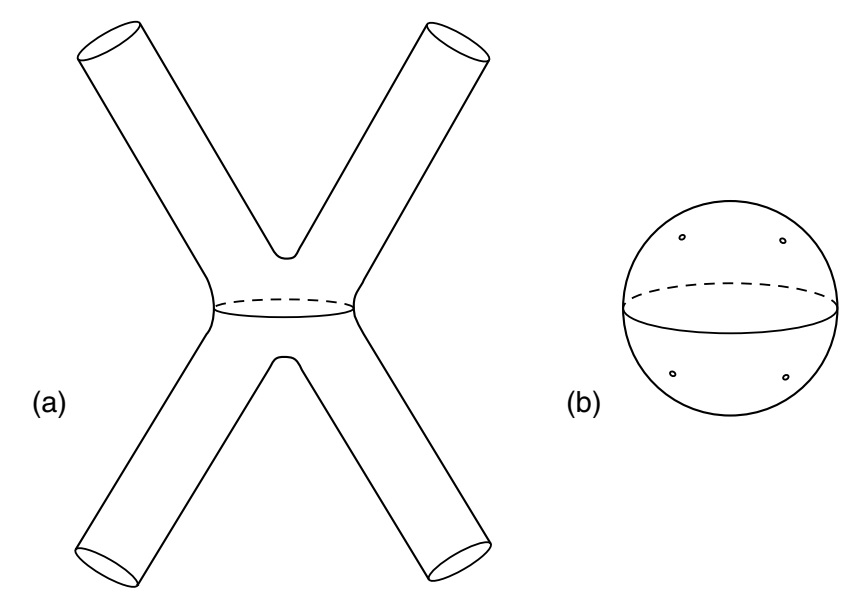
\includegraphics[width=0.8\textwidth,natwidth=645,natheight=450]{Fig3.8.jpg}\\
		\caption{(a) Scattering of four closed strings, with sources approaching $X^{0}=\pm \infty$.(b) Conformally equivalent picture of the four-closed-string scattering: a sphere
			with small holes.}\label{Fig3.8}
	\end{center}
\end{figure}
所以,我们现在来考察图\ref{Fig3.8} 中所示的过程,其中源被拉向了无穷远处. 我们将给出这些源应该如何在路径积分中表示的一个理论. 远离散射过程,弦自由地传播,每个出弦与入弦是一个长圆柱,可以用一个复坐标w描述:
\begin{equation}
-2 \pi t \leq \operatorname{Im} w \leq 0, \quad w \cong w+2 \pi
\end{equation}
圆柱的下端$\operatorname{Im} w=-2 \pi t$,以源为结尾. 上端插入世界面的其余部分,并且圆周是周期Re w方向,对应于散射过程的极限是$t \rightarrow \infty$. 看起来似乎是我们将时空中的长距离与世界面坐标中的长圆柱混淆. 但这将是较为正确的:稍后我们将看到,沿着长时空距离的传播精确来源于这样的世界面,其中圆柱以以上的意义变长.\\
我们在第2章知道,圆柱有一等价描述:

\begin{equation}
z=\exp (-i w), \quad \exp (-2 \pi t) \leq|z| \leq 1
\end{equation}

在这个图景中,长圆柱映射到了单位圆盘,其中外弦态是处在中心的圆. 在内部度规的几何中,图\ref{Fig3.8}a过程现在看起来像是\ref{Fig3.8}b. 在$t \rightarrow \infty$的极限下,小圆收缩成点,而世界面退化至对于每一外态有一类点插入的球面.\\

\begin{figure}
	\begin{center}
		%width=0.8\textwidth,bb=0 0 863 602 
		%1px=0.75pt
		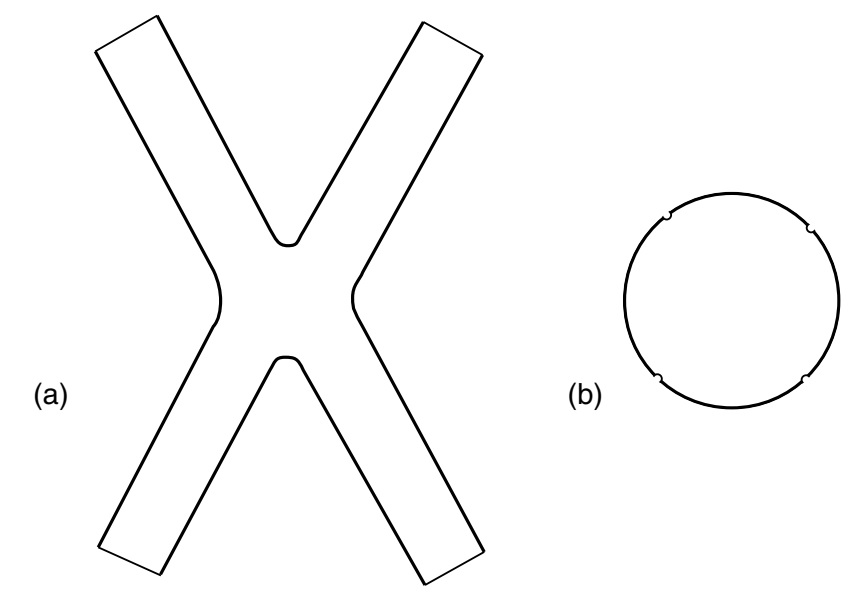
\includegraphics[width=0.8\textwidth,natwidth=645,natheight=450]{Fig3.9.jpg}\\
		\caption{(a) Scattering of four open strings, with sources approaching $X^{0}=\pm \infty$.(b) Conformally equivalent picture: a disk with small dents.}\label{Fig3.9}
	\end{center}
\end{figure}
同样的概念对外开弦态成立. 图\ref{Fig3.9}a过程中的长带可以描述成区域
\begin{equation}
-2 \pi t \leq \operatorname{Im} w \leq 0, \quad 0 \leq \operatorname{Re} w \leq \pi
\end{equation}
其中 $\operatorname{Im} w=-2 \pi t$ 是源,而 $\operatorname{Re} w=0, \pi$ 是端点边界. 在 $z=-\exp (-i w)$下, 这映射成单位圆盘与上半平面的交集. 而在原点处切开了一个小的半圆
\begin{equation}
\exp (-2 \pi t) \leq|z| \leq 1, \quad \operatorname{Im} z \geq 0
\end{equation}
散射过程现在看起来像图\ref{Fig3.9}b. 在$t \rightarrow \infty$的极限下,源收缩成位于(端点)边界上的点.\\
这是我们已经看到的态-算符对应. 每个源变成世界面上的一个定域扰动. 对于一个给定的入弦或出弦,其有D-动量$k^{\mu}$以及内部态j,存在一个由极限过程决定的对应的定域顶角算符 $\mathscr{V}_{j}(k)$ . 出态和入态由 $k^{0}$符号区分; 对于入态 $k^{\mu}=(E, \mathbf{k})$ 和出态 $k^{\mu}=-(E, \mathbf{k})$,图\ref{Fig3.8},\ref{Fig3.9}仅描述了最低阶振幅,但构建是相当普遍的:我们可以将注意力限制在紧致世界面上,其上没有一个趋向无限远处的管,但对于每一外闭弦有一在内部的类点插入. 对于每一外开弦在边界上有一类点插入. 那么一个n点S矩阵元为
\begin{equation}
\begin{array}{l}
S_{j_{1} \ldots j_{n}}\left(k_{1}, \ldots, k_{n}\right) \\
\quad=\sum_{\begin{array}{c}
	\text { compact } \atop \text { topologies }
	\end{array}} \frac{[d X d g]}{V_{\text {diff } \times \text { Weyl }}} \exp \left(-S_{X}-\lambda \chi\right) \prod_{i=1}^{n} \int d^{2} \sigma_{i} g\left(\sigma_{i}\right)^{1 / 2} \mathscr{V}_{j_{i}}\left(k_{i}, \sigma_{i}\right)
\end{array}
\end{equation}
为了使顶点算符插入diff不变,我们沿着世界面对它们积分,在本卷的剩余部分,将看到我们的猜测是正确的. 并且确定了合理的弦S矩阵. \\
依赖于我们所考察的4种理论的那一个,对拓扑的求和可能包含非定向世界面和/或带边世界面. 一般而言,对拓扑的求和不限制在连接世界面;总的过程可能包含两组或多组独立的粒子散射. 将求和约束在连接面上而集中于连接S矩阵是方便的. \\
为了获得连接S矩阵,之后我们必须对世界面所有紧致的、连接的拓扑求和. 在二维中,拓扑的分类是众所周知的. 任何紧致的、连通的、定向的无边二维平面拓扑上等价于有g个柄的球面,g称为平面的亏格. 在图\ref{Fig3.10}中,我们展示了g=0,1,2情形.

\begin{figure}
	\begin{center}
		%width=0.8\textwidth,bb=0 0 890 215
		%1px=0.75pt
		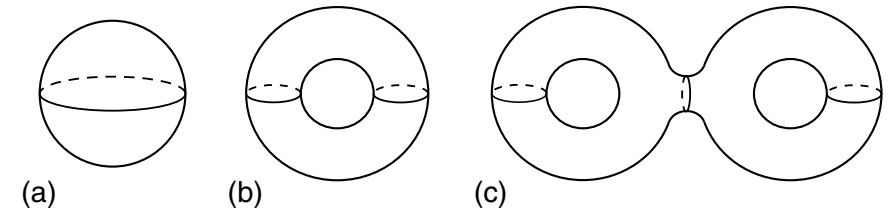
\includegraphics[width=0.8\textwidth,natwidth=667,natheight=161]{Fig3.10.jpg}\\
		\caption{Compact connected closed oriented surfaces of genus (a) 0, (b) 1, (c) 2.}\label{Fig3.10}
	\end{center}
\end{figure}

通过在闭曲面上剪洞可以增加边界. 任何紧致的,连通的,定向二维曲面拓扑等价于有g个柄和b个洞的球面,例如(g,b)=(0,1)是圆盘,(0,2)是圆环,(0,3)是裤子. \\
为了描述非定向曲面,引入十字帽是有用的. 在 面上剪一个洞并将直径相反点等同. 更细致一些,取复坐标,剪出一个略小于单位半径的圆盘,并将通过$z^{\prime}=-1 / \bar{z}$ 定义的相反点粘起来. 由于粘合时反全纯的,所产生的曲面是非定向的. 另外,不像一个边界的情况,十字帽不引入边界或其他定域特征. 由于剪切产生的边界仅是坐标补片的边界,任何紧致连通闭曲面,无论定向还是非定向,总可以在球面上增加g个柄和c个十字帽获得;任何紧致连通曲面可通过增加g个柄,b个边界及c个十字帽获得. 实际上,这些描述有些冗余:无论是无边还是有边情况,通过将求和约束至仅令g和c的一个非零,就能精确获得. 例如(g, b, c) = (0, 0, 1) 是投影平面, (g, b, c) = (0, 1, 1)是Mobius带, (g, b, c) = (0, 0, 2)是Klein瓶, 而一个有十字帽的轮胎面可以通过
(g, b, c) = (0, 0, 3) 或 (g, b, c) = (1, 0, 1)获得, 两个两个十字帽换取一个柄.  Euler数为
\begin{equation}
\chi=2-2 g-b-c
\end{equation}
不同拓扑的数目远小于场论给定阶中不同Feynman图的数目. 例如,在闭定向理论中,在微扰论每一阶,精确存在一个拓扑. 在场论中,图的数目几何增长. 单个弦图包括所有场论图,在不同极限下,柄与它们的圆周相比长得多,我们可以将柄近似为线,而弦图在这个极限下近似为对应的Feynman图.


\section{顶角算子}%{3.6 Vertex operators}

利用态-算符对应,闭弦快子的顶点算符是
\begin{equation}\label{3.6.1}
	\begin{aligned}
		V_{0} &=2 g_{\mathrm{c}} \int d^{2} \sigma g^{1 / 2} e^{i k \cdot X} \\
		& \rightarrow g_{\mathrm{c}} \int d^{2} z: e^{i k \cdot X}:
	\end{aligned}
\end{equation}
我们在映射中引入一个因子$g_c$ ,这是闭弦耦合常数,来自于给过程增加一个额外的弦:我们将顶点算符的归一化用作耦合的定义. 在第二行,我们过渡到了平坦世界面. 顶点算符必须是diff且Weyl不变的,所以,特别地,它在平坦世界面上必须是共形不变的. 为了抵消$d^2 z$的变换,算符必须是权重(1.1)的张量. 通过一个直接的OPE计算,$e^{i k \cdot X}$ 是 $h=\tilde{h}=\alpha^{\prime} k^{2} / 4$ 的张量,所以条件是
\begin{equation}
	m^{2}=-k^{2}=-\frac{4}{\alpha^{\prime}}
\end{equation}
这精确是光锥量子化中所发现的质量.\\
类似地,闭弦的处在第一激发能级的张量态有平坦世界面顶点算符
\begin{equation}
\frac{2 g_{\mathrm{c}}}{\alpha^{\prime}} \int d^{2} z: \partial X^{\mu} \bar{\partial} X^{v} e^{i k \cdot X}:
\end{equation}
与快子顶点算符相关的归一化源于态-算符对应. 我们将在第6章看到,相同的相关归一化从S矩阵的归一化中获得,权重是
\begin{equation}
h=\tilde{h}=1+\frac{\alpha^{\prime} k^{2}}{4}
\end{equation}
所以它们是无质量的,又一次与光锥量子化相符. 为了使其是一个张量,存在进一步的条件,我们将在下面处理.\\

\centerline{\Large Polyakov方法中的顶点算符}

在态-算符映射中,对于任意态,我们有系统的方法写出平坦世界面顶点算符. 既然世界面总能被变成平坦的,原则上,这就是我们需要的全部. 然而现在看来,研究Polyakov体系中的弯曲世界面顶点算符是有用的. 我们将在本节的剩余部分做这件事. 我们使用的方法将有些笨拙,并且不像态-算符映射那样系统,但有些结果是有用的.\\
任何纳入Polyakov路径积分(3.5.5)中的算符必须反应理论的定域diff $\times$ Weyl对称性. 我们还没有具体指出(\ref{3.6.1})的第一行中算符是如何定义在世界面上的. 正如之前关于Weyl反常的讨论,使用自动保护diff不变性,并手动检查Weyl变换是方便的. 对于大部分用途,在文献中使用维数正规化. 然而,对此我们没有大量的需求,所以将不会引入它;相反,我们会推广之前引入的正规序列. 定义一个重整化算符
\begin{equation}\label{3.6.5}
[\mathscr{F}]_{\mathrm{r}}=\exp \left(\frac{1}{2} \int d^{2} \sigma d^{2} \sigma^{\prime} \Delta\left(\sigma, \sigma^{\prime}\right) \frac{\delta}{\delta X^{\mu}(\sigma)} \frac{\delta}{\delta X_{\mu}\left(\sigma^{\prime}\right)}\right) \mathscr{F}
\end{equation}
这里
\begin{equation}
\Delta\left(\sigma, \sigma^{\prime}\right)=\frac{\alpha^{\prime}}{2} \ln d^{2}\left(\sigma, \sigma^{\prime}\right)
\end{equation}
其中$d\left(\sigma, \sigma^{\prime}\right)$ 是 $\sigma$ 和 $\sigma^{\prime}$之间的测地距离. \\
与正规序列相同,(\ref{3.6.5})告诉我们对所有利用 $\Delta\left(\sigma, \sigma^{\prime}\right) $ 收缩 $\mathscr{F}$中的对的方式求和. 在平坦世界面上,$d^{2}\left(\sigma, \sigma^{\prime}\right)=\left|z-z^{\prime}\right|^{2}$并且这退化至共形正规序列,对其我们仔细研究过了. 在弯曲世界面上,它抵消了 $\mathscr{F}$中的场的自收缩的奇异积分. Diff不变性是显然的,但收缩依赖度规. 引入Weyl相关性
\begin{equation}\label{3.6.7}
\delta_{\mathrm{W}}[\mathscr{F}]_{\mathrm{r}}=\left[\delta_{\mathrm{W}} \mathscr{F}\right]_{\mathrm{r}}+\frac{1}{2} \int d^{2} \sigma d^{2} \sigma^{\prime} \delta_{\mathrm{W}} \Delta\left(\sigma, \sigma^{\prime}\right) \frac{\delta}{\delta X^{\mu}(\sigma)} \frac{\delta}{\delta X_{\mu}\left(\sigma^{\prime}\right)}[\mathscr{F}]_{\mathrm{r}}
\end{equation}
第一项成为算符中显式的Weyl相关性.\\
动量为$k_\mu$的态的顶角算符. 在平移下,必须按照与态相同的方式变换,因而形式为$e^{ik\cdot X}$与 $X^\mu$ 相乘的导数.
在Weyl变换下有着不同导数个数的算符不会混合. 所以我们从考察0导数开始,算符(\ref{3.6.1}),Weyl变分来自于显式因子$g^{1/2}$以及(\ref{3.6.7})中所给出的重整化
\begin{equation}\label{3.6.8}
\delta_{\mathrm{W}} V_{0}=2 g_{\mathrm{c}} \int d^{2} \sigma g^{1 / 2}\left(2 \delta \omega(\sigma)-\frac{k^{2}}{2} \delta_{\mathrm{W}} \Delta(\sigma, \sigma)\right)\left[e^{i k \cdot X(\sigma)}\right]_{\mathrm{r}}
\end{equation}
短距离时
\begin{equation}
d^{2}\left(\sigma, \sigma^{\prime}\right) \approx\left(\sigma-\sigma^{\prime}\right)^{2} \exp (2 \omega(\sigma))
\end{equation}
随之
\begin{equation}
\Delta\left(\sigma, \sigma^{\prime}\right) \approx \alpha^{\prime} \omega(\sigma)+\frac{\alpha^{\prime}}{2} \ln \left(\sigma-\sigma^{\prime}\right)^{2}
\end{equation}
在$\sigma^{\prime} \rightarrow \sigma$ 极限下,Weyl变分是非奇异的
\begin{equation}\label{3.6.11}
\delta_{\mathrm{W}} \Delta(\sigma, \sigma)=\alpha^{\prime} \delta \omega(\sigma)
\end{equation}
Weyl变分(\ref{3.6.8})为零的条件就是$k^{2}=4 / \alpha^{\prime}$,正如之上已经推导出的结果.\\

\centerline{\Large off-shell振幅}
考察一个定义off-shell振幅的幼稚尝试,通过取$k^\mu$不在质量面上,这与定域世界面对称性是不相容的. 在位置空间,这意味着弦世界面的一个定域探测,由一在世界面上的插入给定
\begin{equation}\label{3.6.12}
\delta^{D}\left(X(\sigma)-x_{0}\right)=\int \frac{d^{D} k}{(2 \pi)^{D}} \exp \left[i k \cdot\left(X(\sigma)-x_{0}\right)\right]
\end{equation}
由于它包含了全部动量所以是不相容的.\\
从多个角度看,这并不奇怪. \\
首先,之上的讨论,即我们对弦态可使用点源(顶点算符)要求一个极限过程,其显著地将我们约束至面上问题. \\
其次,弦理论包含引力,而在广义相对论中简单off-shell振幅是不存在的,这是因为我们不能不指定探针的位置. 但坐标是非物理的,并且坐标不变off-shell量要复杂得多.\\
第三,在弦论中我们没有引入额外场以测量定域可观察量的自由度(类似于用以探测强相互作用系统的电弱过程):我们必须使用弦本身,或者将我们所讨论的,内禀子理论的其他客体(D膜和孤子).\\
至少在微扰论中是能定义off-shell振幅的. 如果固定规范(对此光锥规范是最简单的)并使用弦源,那么S矩阵可以以更类似于量子场论中的约化公式的方式导出(3.5.5). 其中可以定义有限时间跃迁振幅,然后再取无限时间极限. 附带地,那些尝试将当前讨论与场论关联起来的读者应该注意到路径积分表达式(3.5.5)并不像Green函数而事实上有S矩阵元性质. 场论中类似客体是外传播子被截断的Green函数并且它的外动量被约束在质量面上.\\
定域探测(\ref{3.6.12})的讨论也表明了弦之间接触相互作用的问题,这样相互作用的最简形式将是
\begin{equation}
\int_{M} d^{2} \sigma g(\sigma)^{1 / 2} \int_{M} d^{2} \sigma^{\prime} g\left(\sigma^{\prime}\right)^{1 / 2} \delta^{D}\left(X(\sigma)-X\left(\sigma^{\prime}\right)\right)
\end{equation}
只要世界自交,这不为零. 然而$\delta$函数包含所有动量,就像方程(\ref{3.6.12})中那样. 所以这不是Weyl不变的,弦论的结构相当固定,弦只能以本章开始所描述的方式与弦耦合.\\

\centerline{\Large 无质量闭弦顶点算符}

尽管有些混乱,进一步进行顶点算符的Polyakov处理是有趣的. 不存在一种方式制造精确带有一个导数的世界面标量. 所以下一个情况是两个导数,diff不变的可能情况是
\begin{equation}\label{3.6.14}
	\begin{aligned}
		V_{1}=\frac{g_{\mathrm{c}}}{\alpha^{\prime}} \int d^{2} \sigma g^{1 / 2}\left\{\left(g^{a b} s_{\mu \nu}+i \epsilon^{a b} a_{\mu \nu}\right)\right.&\left[\partial_{a} X^{\mu} \partial_{b} X^{v} e^{i k \cdot X}\right]_{\mathrm{r}} \\
		&\left.+\alpha^{\prime} \phi R\left[e^{i k \cdot X}\right]_{\mathrm{r}}\right\}
	\end{aligned}
\end{equation}
其中$s_{\mu v}, a_{\mu v}$,  $\phi$ 分别是对称矩阵,反对称矩阵和常数. 反对称张量 $\epsilon^{a b}$ 是归一化的, $g^{1 / 2} \epsilon^{12}=1$, 或 $g^{1 / 2} \epsilon^{z \bar{z}}=-i$. 顶点算符中伴随反对称张量中的i可以理解成源于Euclidean延拓,这是因为这一项必有奇数次时间导数(1次) . 这一结果广泛应用于Euclidean作用量与顶点算符. 为了扩张Weyl不变性的分析,我们需要解出高阶的测地距离Weyl相关性(\ref{3.6.11}).
\begin{subequations}\label{3.6.15}
\begin{equation}
\left.\partial_{a} \delta_{\mathrm{W}} \Delta\left(\sigma, \sigma^{\prime}\right)\right|_{\sigma^{\prime}=\sigma}=\frac{1}{2} \alpha^{\prime} \partial_{a} \delta \omega(\sigma)
\end{equation}
\begin{equation}
\left.\partial_{a} \partial_{b}^{\prime} \delta_{\mathrm{W}} \Delta\left(\sigma, \sigma^{\prime}\right)\right|_{\sigma^{\prime}=\sigma}=\frac{1+\gamma}{2} \alpha^{\prime} \nabla_{a} \partial_{b} \delta \omega(\sigma)
\end{equation}
\begin{equation}
\left.\nabla_{a} \partial_{b} \delta_{\mathrm{W}} \Delta\left(\sigma, \sigma^{\prime}\right)\right|_{\sigma^{\prime}=\sigma}=-\frac{\gamma}{2} \alpha^{\prime} \nabla_{a} \partial_{b} \delta \omega(\sigma)
\end{equation}
\end{subequations}
这里$\gamma=-\frac{2}{3}$. 为了之后的参考,我们将其留作参量;第3个方程可以通过第2个方程或第1个方程的梯度得到. 对曲率的变分利用(3.3.5). 对重整化的变分利用(\ref{3.6.7})与(\ref{3.6.15}). 
\begin{equation}\label{3.6.16}
\begin{array}{c}
\delta_{\mathrm{W}} V_{1}=\frac{g_{\mathrm{c}}}{2} \int d^{2} \sigma g^{1 / 2} \delta \omega\left\{\left(g^{a b} S_{\mu v}+i \epsilon^{a b} A_{\mu v}\right)\left[\partial_{a} X^{\mu} \partial_{b} X^{v} e^{i k \cdot X}\right]_{\mathrm{r}}\right. \\
\left.+\alpha^{\prime} F R\left[e^{i k \cdot X}\right]_{\mathrm{r}}\right\}
\end{array}
\end{equation}
其中
\begin{subequations}
\begin{equation}
S_{\mu v}=-k^{2} s_{\mu v}+k_{v} k^{\omega} S_{\mu \omega}+k_{\mu} k^{\omega} s_{v \omega}-(1+\gamma) k_{\mu} k_{v} s_{\omega}^{\omega}+4 k_{\mu} k_{v} \phi
\end{equation}
\begin{equation}
A_{\mu v}=-k^{2} a_{\mu \nu}+k_{v} k^{\omega} a_{\mu \omega}-k_{\mu} k^{\omega} a_{v \omega}
\end{equation}
\begin{equation}
F=(\gamma-1) k^{2} \phi+\frac{1}{2} \gamma k^{\mu} k^{v} s_{\mu v}-\frac{1}{4} \gamma(1+\gamma) k^{2} s_{v}^{v}
\end{equation}
\end{subequations}
在推导Weyl变分(\ref{3.6.16})时,我们进行了分部积分并使用了关系
\begin{equation}\label{3.6.18}
\left[\nabla^{2} X^{\mu} e^{i k \cdot X}\right]_{\mathrm{r}}=i \frac{\alpha^{\prime} \gamma}{4} k^{\mu} R\left[e^{i k \cdot X}\right]_{\mathrm{r}}
\end{equation}
左边本应由于朴素运动方程为零,但这里运动方程乘上了处在同一点的另一算符. 在该情况下成立的广义原理是算符不需要零,但它是不独立的————它可以以该理论中其他定域算符的形式展开. 一般而言,算符的系数依赖于重整化方案;(\ref{3.6.18})可通过取两边的Weyl变分获得.\\
既然$S_{\mu v}, A_{\mu v}$ 和 $F$ 所乘为独立算符,Weyl不变的条件是
\begin{equation}
S_{\mu v}=A_{\mu \nu}=F=0
\end{equation}
为了得到算符数目的精确计数,我们必须注意到不是所有形如(\ref{3.6.14})的$V_1$是独立的. 相反,在
\begin{subequations}\label{3.6.20}
\begin{equation}
s_{\mu v} \rightarrow s_{\mu v}+\xi_{\mu} k_{v}+k_{\mu} \xi_{v}
\end{equation}
\begin{equation}
a_{\mu v} \rightarrow a_{\mu \nu}+\zeta_{\mu} k_{v}-k_{\mu} \zeta_{v}
\end{equation}
\begin{equation}
\phi \rightarrow \phi+\frac{\gamma}{2} k \cdot \xi
\end{equation}
\end{subequations}
利用运动方程(\ref{3.6.18})$V_1$的改变积分为零. 现在这样一个$n^{\mu}$ 满足 $n \cdot k=1$ 和 $n^{2}=0$. 通过约束
\begin{equation}\label{3.6.21}
n^{\mu} s_{\mu v}=n^{\mu} a_{\mu v}=0
\end{equation}
就可以获得一组完备独立算符,这是2D个参量$\xi_{\mu}$ 和 $\zeta_{\mu}$ 的2D个方程;可以证明一个方程和一个参量是平庸的,但方程组(\ref{3.6.21})中的其他方程是非退化的,因而定义了一组独立的顶角算符.
通过使用条件(\ref{3.6.21})并先解出$S_{\mu v} n^{\mu} n^{v}=0$, 之后 $S_{\mu \nu} n^{\mu}=$ $A_{\mu v} n^{\mu}=0$, 最后完全的 $S_{\mu \nu}=A_{\mu \nu}=F=0$, 得到
\begin{subequations}
\begin{equation}\label{3.6.22a}
k^{2}=0
\end{equation}
\begin{equation}\label{3.6.22b}
k^{v} s_{\mu v}=k^{\mu} a_{\mu v}=0
\end{equation}
\begin{equation}\label{3.6.22c}
\phi=\frac{1+\gamma}{4} s_{\mu}^{\mu}
\end{equation}
\end{subequations}
又一次我们发现了质量的条件(\ref{3.6.22a}),这次对应闭弦的第一激发态. 还有偏振垂直于动量的条件(\ref{3.6.22b}),这正是无质量张量场的物理偏振所要求的. 在参考系
\begin{equation}
k^{\mu}=(1,1,0,0, \ldots, 0), \quad n^{\mu}=\frac{1}{2}(-1,1,0,0, \ldots, 0)
\end{equation}
条件(\ref{3.6.21})与(\ref{3.6.22b})暗示了所有0分量与1分量为零. 而(\ref{3.6.22c})固定了$\phi$. 这精确留下了$(D-2)^2$个算符,与光锥规范中所发现的无质量闭弦态数目相同.\\
条件$n^{\mu} s_{\mu v}=n^{\mu} a_{\mu v}=0$被需要以移去零规范类光偏振. 然而矢量$n^\mu$的引入明显破坏了Lorentz不变性. 而这理论只因$n^\mu$的不同选择. 由于(\ref{3.6.20})等而是Lorentz不变的. 为使理论是Lorentz不变的,且有一个正的Hilbert空间范数,(\ref{3.6.20})是重要的. 这些关系是定域时空对称性的特征. 特别地,$\xi_{\mu}$是无穷小时空坐标变换,而$\zeta_{\mu}$是反对称张量场的定域时空对称性. 我们看到了相互作用理论中定域时空对称性的存在. 我们在1.4节讨论过,由于无质量自旋1场和自旋2场的存在,它们必须出现.\\
我们应该提及一个技术上的问题. 不同的重整化方案赋予重整化算符不同的名字. 最常用的方案是维数正规化;这一方案中的算符与之上方案的算符关系为
\begin{subequations}
\begin{equation}
\left[e^{i k \cdot X}\right]_{\mathrm{DR}}=\left[e^{i k \cdot X}\right]_{\mathrm{r}}
\end{equation}
\begin{equation}
\left[\partial_{a} X^{\mu} e^{i k \cdot X}\right]_{\mathrm{DR}}=\left[\partial_{a} X^{\mu} e^{i k \cdot X}\right]_{\mathrm{r}}
\end{equation}
\begin{equation}
\left[\partial_{a} X^{\mu} \partial_{b} X^{v} e^{i k \cdot X}\right]_{\mathrm{DR}}=\left[\partial_{a} X^{\mu} \partial_{b} X^{v} e^{i k \cdot X}\right]_{\mathrm{r}}-\frac{\alpha^{\prime}}{12} g_{a b} \eta^{\mu v} R\left[e^{i k \cdot X}\right]_{\mathrm{r}}
\end{equation}
\begin{equation}
\left[\nabla_{a} \partial_{b} X^{\mu} e^{i k \cdot X}\right]_{\mathrm{DR}}=\left[\nabla_{a} \partial_{b} X^{\mu} e^{i k \cdot X}\right]_{\mathrm{r}}+i \frac{\alpha^{\prime}}{12} g_{a b} k^{\mu} R\left[e^{i k \cdot X}\right]_{\mathrm{r}}
\end{equation}
\end{subequations}
与(\ref{3.6.18})比,我们看到在维数正规化中$\gamma=0$,所以运动方程在正规化算符内成立. 这是一个便利,很多方程简化了. 特别地,在时空规范变化(\ref{3.6.20})中,$\phi$是不变的.\\

\centerline{\Large 开弦顶点算符}

扩展至开弦是直接的,仅给出一些结果,快子顶点算符是
\begin{equation}
g_{\mathrm{o}} \int_{\partial M} d s\left[e^{i k \cdot X}\right]_{\mathrm{r}}
\end{equation}
且对于$k^{2}=1 / \alpha^{\prime}$ 是Weyl不变的. 光子顶点算符是
\begin{equation}
-i \frac{g_{\mathrm{o}}}{\left(2 \alpha^{\prime}\right)^{1 / 2}} e_{\mu} \int_{\partial M} d s\left[\dot{X}^{\mu} e^{i k \cdot X}\right]_{\mathrm{r}}
\end{equation}
其中与快子相关的归一化通过态-算符映射或幺正性获得. i的出现与闭弦情况相同,符号是为了方便. 如果 $k^{2}=0$ 且 $k \cdot e=0 $ ,这个算符是Weyl不变的. 存在等价 $e_{\mu} \cong e_{\mu}+\lambda k_{\mu}$, 这是时空规范变换. 这留下了D-2个横向偏振. \\

\section{弯曲时空中的弦}%{3.7 Strings in curved spacetime}
现在我们来考察一个重要的新课题:在弯曲时空中运动的弦. 我们先来回忆下点粒子情况,它有一个到弯曲时空的自然扩张. 将平坦度规$\eta_{\mu\nu}$替换成一般度规$G_{\mu\nu}$给出作用量
\begin{equation}
S_{\mathrm{pp}}=\frac{1}{2} \int d \tau\left(\eta^{-1} G_{\mu \nu}(X) \dot{X}^{\mu} \dot{X}^{v}-\eta m^{2}\right)
\end{equation}
消掉$\eta$之后,这变成了沿着粒子世界线的不变固有时. 众所周知,它的变分给出测地线方程,代表了在引力场中的粒子运动. 在Polyakov作用量中作一个相同的替换给出
\begin{equation}\label{3.7.2}
S_{\sigma}=\frac{1}{4 \pi \alpha^{\prime}} \int_{M} d^{2} \sigma g^{1 / 2} g^{a b} G_{\mu \nu}(X) \partial_{a} X^{\mu} \partial_{b} X^{v}
\end{equation}
这是一个自然的猜测,但读者可能会提出如下异议. 我们已经了解到了引力子本身就是弦的一个态,一个弯曲时空. 粗略地讲,是引力子的相干背景,因而在弦论中它是弦的一个相干态. 仅在作用量(\ref{3.7.2})中放入弯曲度规看起来似乎不足够弦化. 为了看到为什么它是合理的,考察一个接近平坦的时空
\begin{equation}
G_{\mu v}(X)=\eta_{\mu v}+\chi_{\mu v}(X)
\end{equation}
其中$x_\mu\nu$很小,世界面路径积分中的被积函数是                                        \begin{equation}
S_{\sigma}=\frac{1}{4 \pi \alpha^{\prime}} \int_{M} d^{2} \sigma g^{1 / 2}\left[\left(g^{a b} G_{\mu \nu}(X)+i \epsilon^{a b} B_{\mu \nu}(X)\right) \partial_{a} X^{\mu} \partial_{b} X^{v}+\alpha^{\prime} R \Phi(X)\right.
\end{equation}
$\chi$阶精确是弦的引力子态的顶角算符. 即(\ref{3.6.14})中取
\begin{equation}
\chi_{\mu v}(X)=-4 \pi g_{\mathrm{c}} e^{i k \cdot X} S_{\mu v}
\end{equation}
所以诚然,插入弯曲时空确实与我们已知的发生了联系. 作用量(\ref{3.7.2})可视为通过指数化引力子顶点算符来描述引力子的相干态.\\
这提供一个自然推广: 将其他无质量弦态的背景也纳入进来. 从顶点算符形式(\ref{3.6.14}), 有
\begin{equation}\label{3.7.6}
S_{\sigma}=\frac{1}{4 \pi \alpha^{\prime}} \int_{M} d^{2} \sigma g^{1 / 2}\left[\left(g^{a b} G_{\mu \nu}(X)+i \epsilon^{a b} B_{\mu \nu}(X)\right) \partial_{a} X^{\mu} \partial_{b} X^{v}+\alpha^{\prime} R \Phi(X)\right]
\end{equation}
场$B_{\mu\nu}(x)$是反对称张量,并且伸缩子包含$\Phi$与$G_{\mu\nu}$的对角部分,正如运动方程(\ref{3.6.22c})所暗示的. 作为一个检验,我们来看看时空规范不变性. 在对应于一个场重定义 $X^{\prime \mu}(X)$的路径积分的变量改变下, 若 $G_{\mu v}$与 $B_{\mu v}$按照张量变换,$\Phi$按照标量变换,(\ref{3.7.6})是不变的. 从时空观点看,这是一个坐标变换,这个作用量同样在
\begin{equation}
\delta B_{\mu \nu}(X)=\partial_{\mu} \zeta_{v}(X)-\partial_{v} \zeta_{\mu}(X)
\end{equation}
下不变,这给Lagrangian密度增加了一个全导数. 这是电磁规范变换到有两个反对称指标势的推广. 三指标场强
\begin{equation}
H_{\omega \mu v}=\partial_{\omega} B_{\mu v}+\partial_{\mu} B_{v \omega}+\partial_{v} B_{\omega \mu}
\end{equation}
是不变的. 存在一个类似的到n阶反对称张量势的推广,其在超弦中扮演了重要角色.\\
这个理论因而只依赖于度规和其他场所构建的规范不变量. 可以认为场$X^\mu$是流行上的坐标,这称为靶空间,因而$X^\mu$定义了一个嵌入
\begin{equation}
\text { 世界面 } \rightarrow \text { 靶 }
\end{equation}
在弦理论中,靶空间是时空本身. 诸如(\ref{3.7.2})的场论,其中动能项是场相关的,因而场空间实际上是弯曲流形,由于历史原因而被称为非线性$\sigma$模型,它在粒子物理与量子场论中有很多应用. 例如,中性以及带电$\pi$介子场可很好地近似为群流形SU(2)上的坐标. \\
非线性 $\sigma$模型不再是$X^\mu$的二次型,所以路径积分现在是一个相互作用二维量子场论. 将路径积分在经典解$X^{\mu}(\sigma)=x_{0}^{\mu}$ 附近展开,即$X^{\mu}(\sigma)=x_{0}^{\mu}+Y^{\mu}(\sigma)$
\begin{equation}
\begin{aligned}
G_{\mu \nu}(X) \partial_{a} X^{\mu} \partial_{b} X^{v} &=\left[G_{\mu \nu}\left(x_{0}\right)+G_{\mu v, \omega}\left(x_{0}\right) Y^{\omega}\right.\\
+&\left.\frac{1}{2} G_{\mu v, \omega \rho}\left(x_{0}\right) Y^{\omega} Y^{\rho}+\ldots\right] \partial_{a} Y^{\mu} \partial_{b} Y^{v}
\end{aligned}
\end{equation}
展开中第一项是场$Y^\mu$的2次动能项;接下来一项是立方相互作用,依次类推. 展开中的耦合常数,$G_{\mu \nu, \omega}\left(x_{0}\right)$
等,包含了 $x_{0}$处的导数. 在曲率的特征半径为 $R_{\mathrm{c}}$的靶空间中, 度规的导数是 $R_{\mathrm{c}}^{-1}$阶的. 因而,该理论中有效无量纲耦合是 $\alpha^{1 / 2} R_{\mathrm{c}}^{-1}$. 如果曲率半径 $R_{\mathrm{c}}$ 远大于弦的特征长度,那么这个耦合是弱的,并且二维场论的微扰论是个有用的工具. 注意到在同一体系下我们也可采用其他工具. 由于特征长度远大于弦,我们可以忽略弦的内部结构并使用低能有效场论. 正如我们所要看到的,在决定场论的低能有效作用量时,弦论进入了. 当约束我们的注意力至无质量背景时, 我们暗含使用$\alpha^{\prime 1 / 2} R_{\mathrm{c}}^{-1} \ll 1$ :当波长大于弦尺度时,有质量弦态没有被创造.\\
非线性$\sigma$模型(\ref{3.7.2})是可重整理论:场$Y^\mu$有量纲0,因而相互作用都有量纲2. 然而耦合,即度规展开式的系数,在数值上是无限大(除非某些对称性限制了度规的形式). 实际上将度规函数本身,而非它的展开系数,定义理论的耦合更有用些.\\

\centerline{\Large Weyl不变性}

我们已经强调了Weyl不变性对弦论的一致性是重要的. 仅当二维量子场论是Weyl不变的,作用量(\ref{3.7.6})将定义一个一致的弦论. 这个作用量碰巧是在刚性Weyl变换下经典不变的最普遍作用量,刚性变换中 $\delta \omega$ 独立于 $\sigma$. 这很容易看到:在一个刚性Weyl变换下,有 $n$ 个导数的收缩将正比于 $2-n $. 当然,考察定域Weyl变换也有必要,在这个域,(\ref{3.7.6})中的 $G_{\mu v}$ 和 $B_{\mu v}$ 是不变的,但 $\Phi$ 项不是, 并且包含了对Weyl变换的量子贡献. $B_{\mu v}$ 和 $\Phi$ 很小, $G_{\mu v}$ 接近 $\eta_{\mu v}$的极限下, 我们可以使用上述结果寻找Weyl变换.  写成$S_{\sigma}=S_{\mathrm{P}}-V_{1}+\ldots$, 其中 $S_{\mathrm{P}}$ 是平坦空间作用量, $V_{1}$ 是顶点算符(\ref{3.6.14}). 那么
\begin{subequations}
\begin{equation}
G_{\mu v}(X)=\eta_{\mu v}-4 \pi g_{\mathrm{c}} s_{\mu \nu} e^{i k \cdot X}
\end{equation}
\begin{equation}
B_{\mu \nu}(X)=-4 \pi g_{\mathrm{c}} a_{\mu \nu} e^{i k \cdot X}
\end{equation}
\begin{equation}
\Phi(X)=-4 \pi g_{\mathrm{c}} \phi e^{i k \cdot X}
\end{equation}
\end{subequations}
我们当然可以取动量不同的顶点算符的线性组合. 那么,到一阶,Weyl变换在(\ref{3.6.16})中被给出,方便起见,我们取$\gamma=0$的重整化方案,像(\ref{3.4.6})中那样将Weyl变换与$T_a^a$ 关联起来给出
\begin{equation}
T^{a}{ }_{a}=-\frac{1}{2 \alpha^{\prime}} \beta_{\mu v}^{G} g^{a b} \partial_{a} X^{\mu} \partial_{b} X^{v}-\frac{i}{2 \alpha^{\prime}} \beta_{\mu v}^{B} \epsilon^{a b} \partial_{a} X^{\mu} \partial_{b} X^{v}-\frac{1}{2} \beta^{\Phi} R
\end{equation}
其中,至$\chi_{\mu \nu}, B_{\mu \nu}$ and $\Phi$ 的线性阶.
\begin{subequations}\label{3.7.13}
\begin{equation}
\beta_{\mu v}^{G} \approx-\frac{\alpha^{\prime}}{2}\left(\partial^{2} \chi_{\mu \nu}-\partial_{v} \partial^{\omega} \chi_{\mu \omega}-\partial_{\mu} \partial^{\omega} \chi_{\omega v}+\partial_{\mu} \partial_{v} \chi_{\omega}^{\omega}\right)+2 \alpha^{\prime} \partial_{\mu} \partial_{v} \Phi
\end{equation}
\begin{equation}
\beta_{\mu \nu}^{B} \approx-\frac{\alpha^{\prime}}{2} \partial^{\omega} H_{\omega \mu \nu}
\end{equation}
\begin{equation}
\beta^{\Phi} \approx \frac{D-26}{6}-\frac{\alpha^{\prime}}{2} \partial^{2} \Phi
\end{equation}
\end{subequations}
在$\beta^{\Phi}$中, 我们引入了3.4节所发现的平坦时空反常,其中暗含了来自于鬼场的正比于26的贡献. 符号 $\beta$ 用于 $T^{a}{ }_{a}$ 中的系数是因为这些显然是重整化群beta函数, 控制了物理对世界面尺度的依赖. 我们将进一步讨论这个.
Weyl 反常 (\ref{3.7.13}) 有来自高阶场的进一步贡献. 例如,将路径积分展开至 (3.7.10)中三次项的二阶,当两个相互作用彼此接近会产生发散. 它们的 OPE 包含形式为 $|z|^{-2} \partial X^{\mu} \bar{\partial} X^{v}$ 乘以 $G_{\alpha \beta} $ 导数的平方的奇异性.  Diff不变要求这个积分以不变距离的形式, $|z| \exp (\omega)>a_{0} $被截断. 这引入了对度规尺度的依赖性,$\ln z_{\min }=-\omega+\ln a_{0}$. Weyl 变分 $\beta_{\mu v}^{G}$
因而得到正比于 $O\left(G_{\alpha \beta, \gamma}\right)^{2}$ 的贡献,其组合线性二阶导数项以构成时空Ricci张量.\\
我们再次不讨论细节,但引用保留所有项直至两个导数的结果
\begin{subequations}\label{3.7.14}
\begin{equation}
\beta_{\mu \nu}^{G}=\alpha^{\prime} \boldsymbol{R}_{\mu v}+2 \alpha^{\prime} \nabla_{\mu} \nabla_{v} \Phi-\frac{\alpha^{\prime}}{4} H_{\mu \lambda \omega} H_{v}{ }^{\lambda \omega}+O\left(\alpha^{\prime 2}\right)
\end{equation}
\begin{equation}
\beta_{\mu \nu}^{B}=-\frac{\alpha^{\prime}}{2} \nabla^{\omega} H_{\omega \mu v}+\alpha^{\prime} \nabla^{\omega} \Phi H_{\omega \mu \nu}+O\left(\alpha^{\prime 2}\right)
\end{equation}
\begin{equation}
\beta^{\Phi}=\frac{D-26}{6}-\frac{\alpha^{\prime}}{2} \nabla^{2} \Phi+\alpha^{\prime} \nabla_{\omega} \Phi \nabla^{\omega} \Phi-\frac{\alpha^{\prime}}{24} H_{\mu \nu \lambda} H^{\mu \nu \lambda}+O\left(\alpha^{\prime 2}\right)
\end{equation}
\end{subequations}
(\ref{3.7.14})中的几项可以从线性近似(\ref{3.7.13})中辨认出来,但现在在时空坐标的改变下变得协变. 时空Ricci张量是 $\boldsymbol{R}_{\mu v}$, 与世界面Ricci 张量 $R_{a b} $区分. 有更多导数的项是世界面 $\alpha^{1 / 2} R_{\mathrm{c}}^{-1}$ 展开中的高阶. 进行高阶Weyl反常计算的最有效方法不是我们所描述的,而是维数正规化. \\
世界面是Weyl不变的,因而条件是
\begin{equation}
\beta_{\mu v}^{G}=\beta_{\mu v}^{B}=\beta^{\Phi}=0
\end{equation}
它们是看起来合理的运动方程. 方程$\beta_{\mu v}^{G}=0$ 类似于源项来自于反对称张量场和伸缩子场的 Einstein方程. $\beta_{\mu v}^{B}=0$ s是Maxwell方程的反对称张量推广,决定了场强的发散.\\

\centerline{\Large 背景}
场方程的另一定性特征现在能够理解了:场$\Phi$总存在微分,所以存在在$\Phi$的x无关偏移下的不变. 这是因为这样的偏移为作用量(\ref{3.7.6})造成的改变是正比于Euler数的一项,因而并不影响类似Weyl不变的定域性质.
特别地,背景
\begin{equation}
G_{\mu v}(X)=\eta_{\mu \nu}, \quad B_{\mu \nu}(X)=0, \quad \Phi(X)=\Phi_{0}
\end{equation}
对于任何常数$\Phi_0$是Weyl不变的,这正是平坦时空作用量(3.2.2). 其中
\begin{equation}
\lambda=\Phi_{0}
\end{equation}
$\lambda$决定弦之间的耦合强度. 但我们现在看到这个参量的不同值并不意味着存在不同的弦理论.  $\lambda$不同值并不对应不同的理论,而是对应单个理论中不同的背景. 出现在 Nambu-Goto 和 Polyakov 作用量中的其他参量, Regge 斜率 $\alpha^{\prime}$, 也不是真的自由参量,因为它是有量纲的. 它定义了长度单位,并可以吸收进 $X^{\mu}$的定义中. \\
改变世界面作用量中的场 $G_{\mu v}, B_{\mu v}$, 和 $\Phi$ 似乎会,以二维的观点看,给出一个新的理论. 从纯弦论的观点看,这仅是在同一理论下处在不同的背景:一个不同的态下观察. 这是使弦论有吸引力的特征之一. 在标准模型中,以及在大多数量子场论框架下统一标准模型的尝试中,存在很多不由理论决定的常数;这些常数的任何值给出一个相容的理论. 在弦论中,不存在这样的自由参量————耦合常数依赖于态且原则上由动力学决定. 当然,现在这仅是把困难移到了别处,因为我们对动力学的理解程度不足以知道背景的值.\\
令人惊讶的是,Einstein方程在一个看起来不同寻常的地方出现了,作为二维场论Weyl不变的条件. 弦论提供了这两个概念的联系. 同样引人注意的是,弦仅在满足合适场方程的背景中相容的传播. 这平行于我们早期的仅面上顶角算符有意义的发现.\\
另一发现:条件 $D=26$ 来自 $T^{a}{ }_{a}$中的R项. 在非线性sigma 模型中,这被推广至 $\beta^{\Phi}=0$. 我们在 (3.7.14c)中看到  $\beta^{\Phi}$ 中的领头阶正比于 $D-26$ ,但存在包含场梯度的修正. 显然,如果场不是常数,我们有另一 $D$值. 这是正确的,尽管我们不能真的从(3.7.14c)中得到它,因为这是在近似 $\alpha^{\prime 1 / 2} R_{\mathrm{c}}^{-1} \ll 1$ 下导出的,而其中 $\beta^{\Phi}$ 的修正很小. 事实上, $D \neq 26$ 的精确解是知道的. 我们现在给出一个例子:
\begin{equation}\label{3.7.18}
G_{\mu \nu}(X)=\eta_{\mu \nu}, \quad B_{\mu \nu}(X)=0, \quad \Phi(X)=V_{\mu} X^{\mu}
\end{equation}
如果
\begin{equation}
V_{\mu} V^{\mu}=\frac{26-D}{6 \alpha^{\prime}}
\end{equation}
beta函数(\ref{3.7.14})为零. \\
这个结果实际上是精确的,因为场(\ref{3.7.18})对$X^\mu$是常数或线性的,所以世界面路径积分仍然是Gauss的. 变分 $g_{a b}$ 以决定这个理论的 $T_{a b}$ , 发现他正是伸缩子 CFT,其中心荷 $c=D+6 \alpha^{\prime} V_{\mu} V^{\mu}$ 在条件 (3.7.19)下确定是26. 由于$\Phi$ 必须有一个大的梯度以改变D,这个CFT并不描述我们近似平坦且齐次的4维时空,但它可能有宇宙学上的应用. 这个CFT同样是重要的,因为D=1和D=2的情况对弦论是足够简单以至于精确可解的.\\

\centerline{\Large 时空作用量}

场方程(3.7.15)可从时空作用量
\begin{equation}
	\begin{aligned}
		\boldsymbol{S}=\frac{1}{2 \kappa_{0}^{2}} \int d^{D} x(-G)^{1 / 2} e^{-2 \Phi}[& \frac{2(D-26)}{3 \alpha^{\prime}}+\boldsymbol{R}-\frac{1}{12} H_{\mu \nu \lambda} H^{\mu \nu \lambda} \\
		&\left.+4 \partial_{\mu} \Phi \partial^{\mu} \Phi+O\left(\alpha^{\prime}\right)\right]
	\end{aligned}
\end{equation}
归一化常数$k_0$不由场方程决定,并且由于它可以通过$\Phi$的重定义被改变,因而没有物理重要性. 可以证明
\begin{equation}
\begin{aligned}
\delta \boldsymbol{S}=-\frac{1}{2 \kappa_{0}^{2} \alpha^{\prime}} & \int d^{D} x(-G)^{1 / 2} e^{-2 \Phi}\left[\delta G_{\mu v} \beta^{G \mu v}+\delta B_{\mu v} \beta^{B \mu v}\right.\\
&\left.+\left(2 \delta \Phi-\frac{1}{2} G^{\mu v} \delta G_{\mu \nu}\right)\left(\beta_{\omega}^{G \omega}-4 \beta^{\Phi}\right)\right]
\end{aligned}
\end{equation}
注意,这是控制低能时空场的有效作用量. \\
做如下形式的场重定义通常是有用的:
\begin{equation}
\tilde{G}_{\mu \nu}(x)=\exp (2 \omega(x)) G_{\mu \nu}(x)
\end{equation}
这是时空Weyl变换,由$\tilde{G}_{\mu \nu}$构造的Ricci标量是
\begin{equation}
\tilde{\boldsymbol{R}}=\exp (-2 \omega)\left[\boldsymbol{R}-2(D-1) \nabla^{2} \omega-(D-2)(D-1) \partial_{\mu} \omega \partial^{\mu} \omega\right]
\end{equation}
对于特殊情况D=2,这是Weyl变换(3.3.5). 令$\omega=2\left(\Phi_{0}-\Phi\right) /(D-2)$,并定义
\begin{equation}
\tilde{\Phi}=\Phi-\Phi_{0}
\end{equation}
其有一个归零的期望值. 作用量变成
\begin{equation}
\begin{aligned}
\boldsymbol{S}=& \frac{1}{2 \kappa^{2}} \int d^{D} X(-\tilde{G})^{1 / 2}\left[-\frac{2(D-26)}{3 \alpha^{\prime}} e^{4 \tilde{\Phi} /(D-2)}+\tilde{\boldsymbol{R}}\right.\\
&\left.-\frac{1}{12} e^{-8 \tilde{\Phi} /(D-2)} H_{\mu \nu \lambda} \tilde{H}^{\mu \nu \lambda}-\frac{4}{D-2} \partial_{\mu} \tilde{\Phi} \tilde{\partial}^{\mu} \tilde{\Phi}+O\left(\alpha^{\prime}\right)\right]
\end{aligned}
\end{equation}
其中波浪号是作为一个提醒:指标是被 $\tilde{G}^{\mu \nu}$所上升的. 以 $\tilde{G}_{\mu v}$的形式, 引力 Lagrangian 密度取标准形式  $(-\tilde{G})^{1 / 2} \tilde{\boldsymbol{R}} / 2 \kappa^{2} $ ,常数$\kappa=\kappa_{0} e^{\Phi_{0}}$ 是观察到的引力耦合常数.
其自然有值
\begin{equation}
\kappa=\left(8 \pi G_{\mathrm{N}}\right)^{1 / 2}=\frac{(8 \pi)^{1 / 2}}{M_{\mathrm{P}}}=\left(2.43 \times 10^{18} \mathrm{GeV}\right)^{-1}
\end{equation}
普遍地, $G_{\mu v}$ 被称为sigma模型度规或弦度规,而$\tilde{G}_{\mu v}$ 称为 Einstein度规. 由于来自于伸缩子交换的力,不存在等效原理. 因而没办法挑出度规的一个优先定义. 继续向前,在弦论中存在高阶效应可以赋予伸缩子质量以及一个有限范围————这是好事,因为等效原理确实以非常高的精度成立.\\
注意到出现在作用量(3.7.20) 中的伸缩子在总因子 $e^{-2 \Phi}$中,并且在其他地方总是以微分形式出现. 这与如下事实是一致的:给伸缩子增加一个总常数对Weyl反常没有影响. 从时空的观点看,这给作用量乘上了一个常数,但不影响运动方程. 它也反应了这样的事实:在量子场论中,以耦合常数g作为一个总因子 $g^{-2}$出现的方式重调场是可能的, 且在弦论中则是 $e^{-2 \Phi}$. 例如,Yang-Mills作用量通常以如下形式引入
\begin{subequations}
\begin{equation}
\boldsymbol{S}=-\frac{1}{4} \int d^{D} x \operatorname{Tr}\left(F_{\mu v} F^{\mu v}\right)
\end{equation}
\begin{equation}
F_{\mu v}=\partial_{\mu} A_{v}-\partial_{v} A_{\mu}-i g\left[A_{\mu}, A_{v}\right]
\end{equation}
\end{subequations}
通过定义
\begin{equation}
g A_{\mu}=A_{\mu}^{\prime}, \quad g F_{\mu v}=F_{\mu v}^{\prime}
\end{equation}
g从场强,协变导数以及规范变换中被消除了,而以 $g^{-2}$出现在作用量中. 在弦论中,当作用量被写成出现在世界面上的场的形式,这是成立的.  就像到达(3.7.25)所要做的. 那么这不再成立.\\
当g仅在作用量的归一化中出现时,每个传播子包含一个 $g^{2}$ 因子,每个相互作用包含 $g^{-2}$. 不难证明对有效作用量的 L -圈 贡献中传播子比顶点多 $L-1$个,所以重调为  $g^{2(L-1)} $ . 在弦论中,这是$e^{-\chi \Phi}$, 也是我们所期待的.\\
背景的讨论可扩至开弦. 我们已经看到开弦顶点算符是沿着边界被积分的,所以开弦场作为边界项出现在sigma模型作用量中.
\\

\centerline{\Large 紧致化与CFT}
目前为止研究的四种弦论(有没有边界,定向或非定向)有一些共同的特征:一个很好的特征是广义相对论的自动包含,也存在几个坏特征:26维的需要,快子的存在,以及频谱中没有Fermion. 然而,广义相对论的出现给出了额外维的一种自然的解释,时空的几何是动力学的,不是固定的. 平坦时空仅是场方程众多解中的一个. 可能存在一些解,其中有些维很大且平坦,而其他的很小且高度蜷曲. 度规是
\begin{equation}\label{3.7.29}
g_{M N}=\left[\begin{array}{cc}
\eta_{\mu v} & 0 \\
0 & g_{m n}\left(x^{p}\right)
\end{array}\right]
\end{equation}
我们已经把26个坐标$M,N=0,\cdots,25$分成四个时空坐标 $\mu, v=0, \ldots, 3$ 和 22 个内部坐标 $m, n, p=4, \ldots, 25$ . 度规 (\ref{3.7.29}) 在四维是平坦的,但在22维是卷曲的. 假定内部空间紧致. 一个例子:若伸缩子场是一个常数,背景场方程 (3.7.15) 满足 $\alpha^{\prime}$阶 , 反对称张量是零, 内部空间是Ricci平坦的,  $\boldsymbol{R}_{m n}=0$.\\
换句话说,时空形式为 $M^{d} \times K$,其中 $M^{d}$ 是$d$维 Minkowski空间, $K$ 是某种 $(26-d)$ 维紧致Riemannian空间. 在这样的时空长度远大于k的大小上的物理与d维Minkowski时空的物理是相同的. 存在很好的理由独立于弦论考察我们时空是这一形式的可能性.\\
我们可进一步推广这个概念. 基本的物理相容性条件就那么几个. 我们要求Lorentz不变性,要求量子力学几率正定且守恒————迄今为止, 弦论中似乎没有什么要求标准量子力学基础被修正,尽管对其有不同认识将是有趣的,尽管这些条件是简单的. 在规范理论,引力和弦论之间存在一些不安. 在显然协变规范中存在着必须从物理振幅中退耦负范类时激发. 在光锥规范中,内积是正定的\\
因而一个必要条件是二维diff不变性,使得非物理振子仅是坐标系统的振子. Weyl不变性是一个更加技巧的要求:当Weyl不变丢失所产生的额外自由度闭坐标系统振子.\\
我们也将做一个额外的技巧性假定: 出现在世界面作用量中的嵌入时,$X_0$   仅在
\begin{equation}\label{3.7.30}
-\frac{1}{4 \pi \alpha^{\prime}} \int_{M} d^{2} \sigma g^{1 / 2} g^{a b} \partial_{a} X^{0} \partial_{b} X^{0}
\end{equation}
例如,在sigma模型中,这意味着场是静态的, $G_{0 \mu}=\eta_{0 \mu}$ 且 $B_{0 \mu}=0 $. 这一假定算不上一个约束. 如果感兴趣的是静态, $(3.7 .30)$ 足够. 时间相关背景也肯定是重要的, 但除了在时间尺度就是弦尺度的极度情况下,它们可以用低能有效场论来分析. 做出假定$(3.7 .30)$ 的原因是要把主要问题,$X^0$的错号特征, 放在一个明显的形式中. \\
要求体现定域不变性导致了对更加普遍弦论的如下提议:将 25 空间场 $X^{\mu}$ 替换成任何有 $c=\tilde{c}=25$的幺正CFT. 这确保了全二维理论,包含 $X^{0}$ 和鬼,可以以一种方式与一弯曲(diff $\times$ Weyl)度规耦合. 幺正(正定内积)条件是必须的,因为仅存在足够的定域规范对称性以移除非物理$X^{0}$激发 . 世界面内积在这里是相关的,因为它在单粒子扇区变成了时空内积,在第二卷. 我们将看到,进一步推广是可能的, 同时扩大了定域对称群与非物理激发的集合.   \\                                                   \\
如果我们感兴趣的是低能物理看起来像四维的,我们保持自由场 $X^{\mu}$ , $\mu=0,1,2,3$, 而将剩余的$X^{\mu}$ 替换成 $c=\tilde{c}=22$的紧致幺正CFT. 对于紧致化,我们意指频谱是离散的,正如有限体积内的量子场论. 存在某些尝试以构建所有的CFT,我们将在15章描述. 
所有这些理论都有快子,内部CFT中的幺正态 $|1\rangle$ 与四维CFT基态 $|0 ; k\rangle$的乘积.\\
我们所作的推广有多大?如果定域对称性是唯一显著的约束,我们可以在世界面上随意引入场,其有不同的世界面和时空量子数. 这似乎使得我们我们远离了原始的26维$X^\mu$场. 然而在二维中,在看似不同的量子场论之间存在很多等价性,使得情况不那么显然. \\
一般而言,所有弦论基本与不同CFT. 但是相同的世界面对称性以及拓扑是统一理论的不同基态. 这引起了语义上的问题:我们通常指世界面上拉式量不同的弦为不同的理论. 尽管它们可能只是同一理论的不同真空. 14章我们将进一步处理.我们将看到所有的弦论表现为单个理论的真空.
